%\documentclass[handout]{beamer}
%\documentclass{beamer}
\documentclass[aspectratio=169]{beamer}
%\documentclass{beamer}

%\usepackage{beamerthemesplit}
%\usepackage{logicthemelive}
\usepackage{cite}
%\usepackage{enumitem}
\usepackage{pgf}
\usepackage{tikz}
\usepackage{graphicx}
\usepackage{datatool}
\usepackage{dataplot}
\usepackage{xcolor}
\usetikzlibrary{calc,through,decorations.pathmorphing}
\usetikzlibrary{decorations.text}
\usetikzlibrary{trees}
\usetikzlibrary{fit}
\usetikzlibrary{backgrounds}
\usetikzlibrary{positioning}
\usetikzlibrary{shapes,arrows}
\usetikzlibrary{shadows}
\usetikzlibrary{calendar}
%\usepackage[cmex10]{amsmath}
%\usepackage{array}
\usepackage{ctable}
\usepackage{dcolumn}
\usepackage{mdwmath}
\usepackage{mdwtab}
\usepackage{setspace}
\usepackage{fancyhdr}
%\usepackage{electComp}
%\usepackage{amsmath}
\usepackage{textcomp}

\title[125 years of data]{\huge 125 years of data}
%\author{Dr David Hume}
\subtitle{\tiny EEA -- 21st June, 2013} % (optional)
\author[David Hume]{\footnotesize David Hume\normalsize  \\ \tiny {\texttt{david.hume@ea.govt.nz}} \\ \tiny Market Performance team, Electricity Authority of New Zealand}
%\institute{\tiny Electricity Authority of New Zealand}
\date{}



\begin{document}

\frame{\titlepage}


\frame
{\frametitle{My home energy monitor -- Current Cost + RaspberryPi}
\begin{columns}[t]
  \column[T]{5cm}
  Current Cost energy monitor
      \includegraphics[width=5.0cm]{wpid-20130116_080753.jpg} 
  \column[T]{5cm}
  \vspace{5mm}
  Raspberry Pi computer
  \includegraphics[width=5.0cm]{RaspberryPi.jpg}
  \begin{itemize}
  \item Python script
  \item MySQL database
  \item iPython
  \end{itemize}
\end{columns}
}

\frame
{\frametitle{My home energy monitor -- weeks worth of data}
\begin{center}
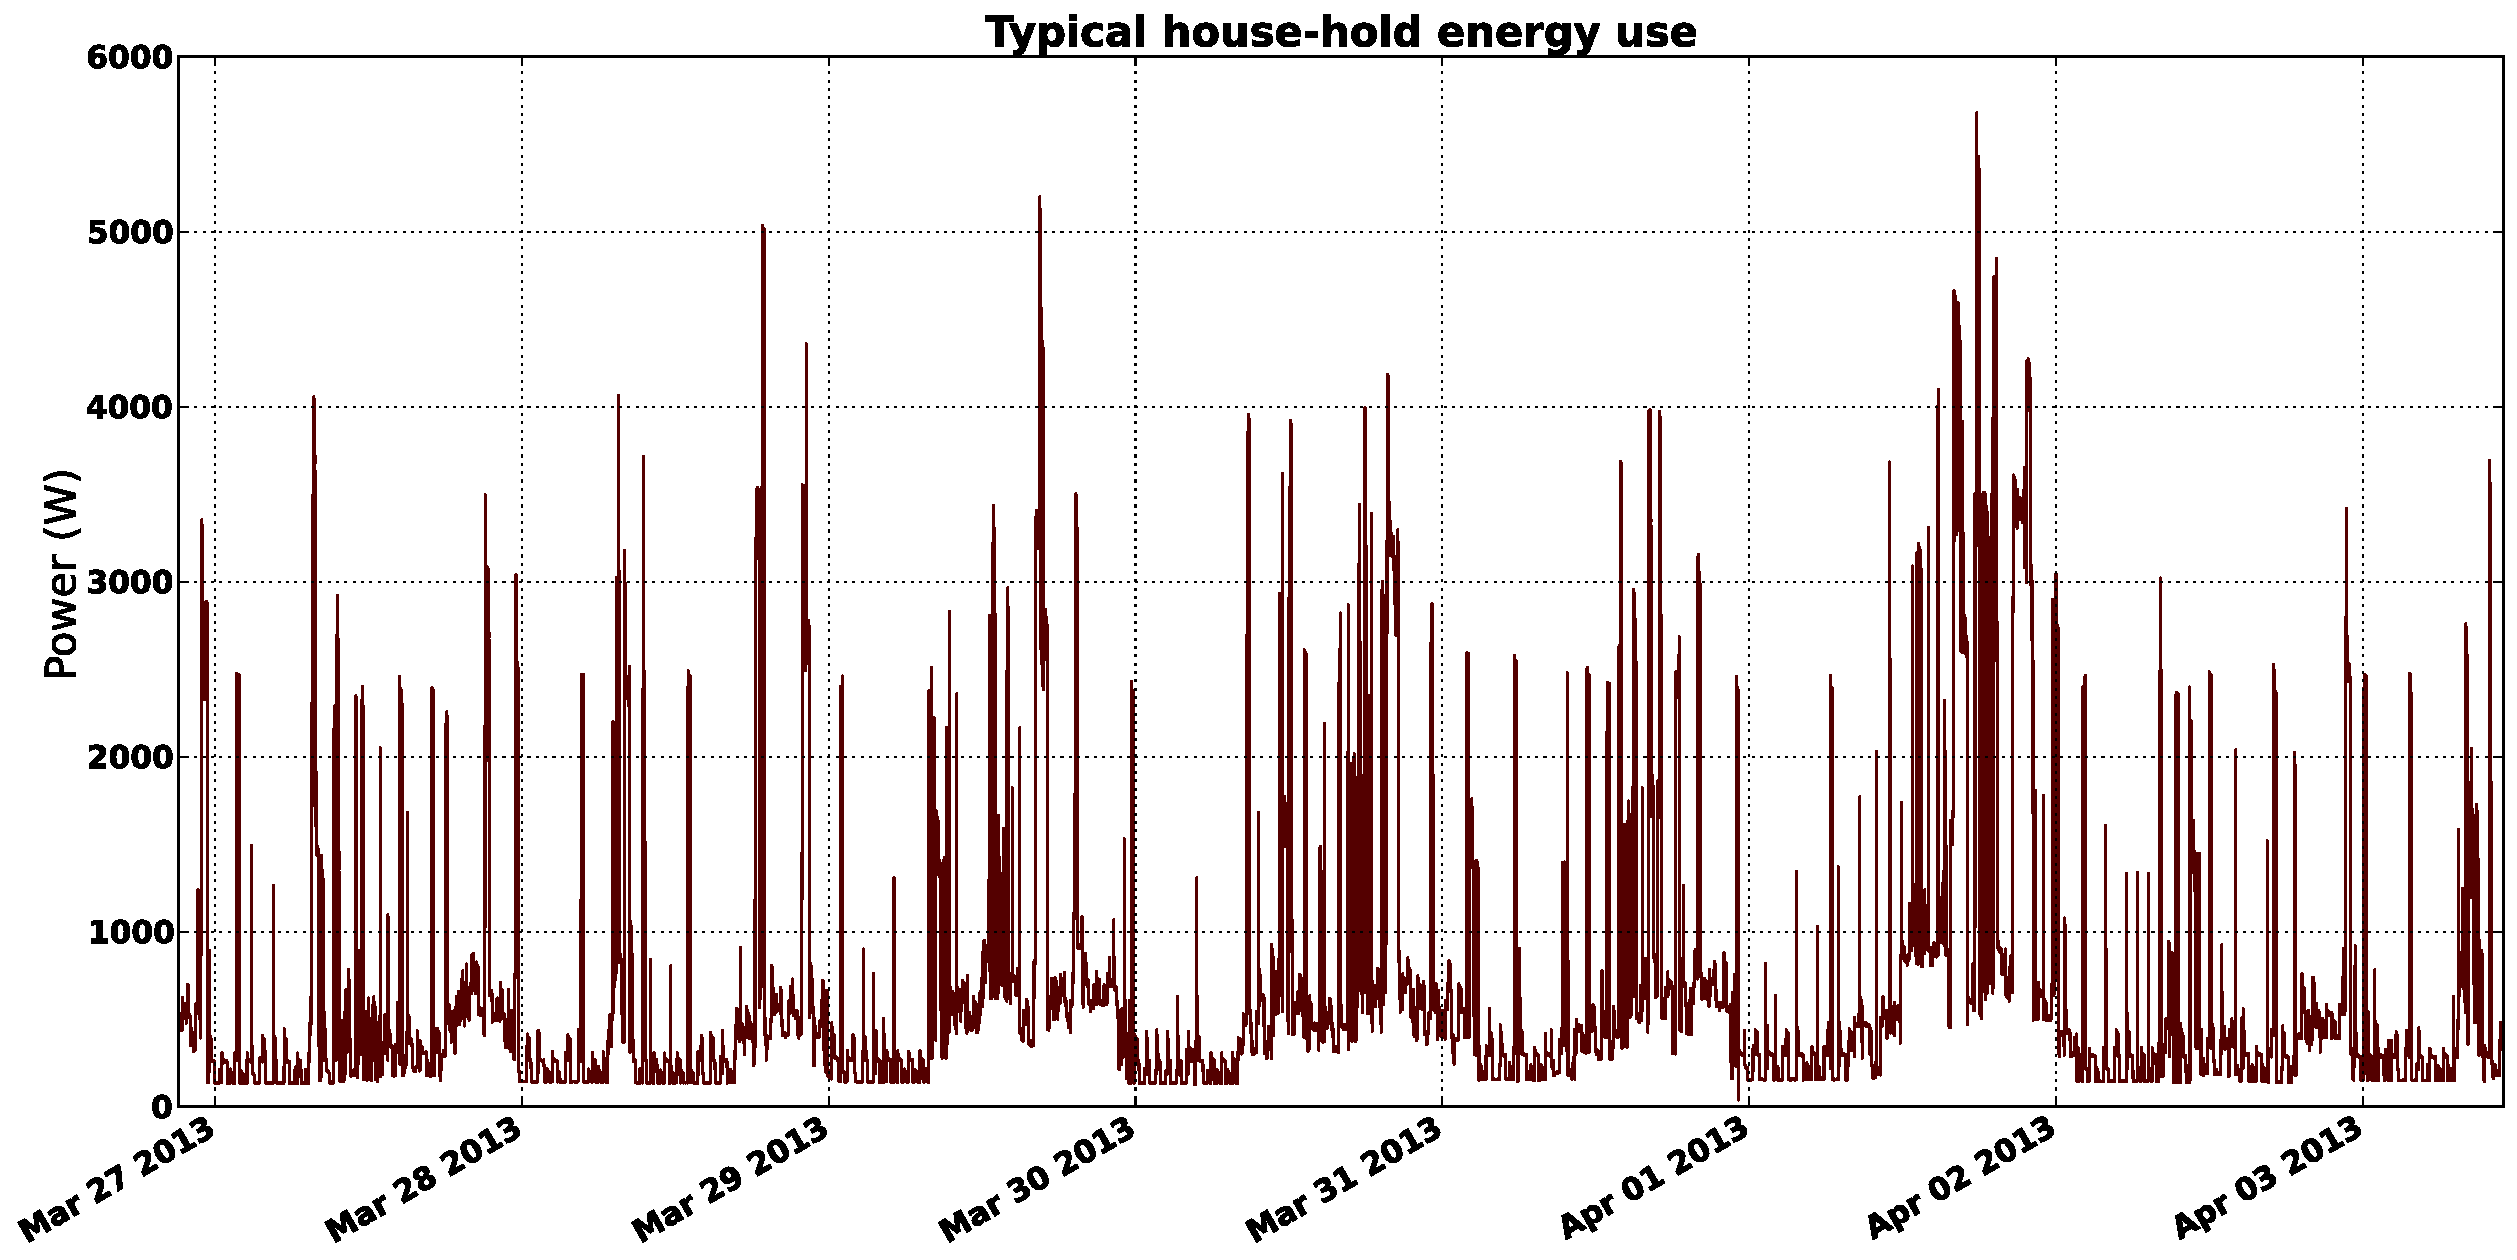
\includegraphics[width=14cm]{./notebooks/125_years_of_data_files/125_years_of_data_fig_03.pdf} 
\end{center}
}


\frame
{\frametitle{Home energy monitoring -- a high usage day}
\begin{center}
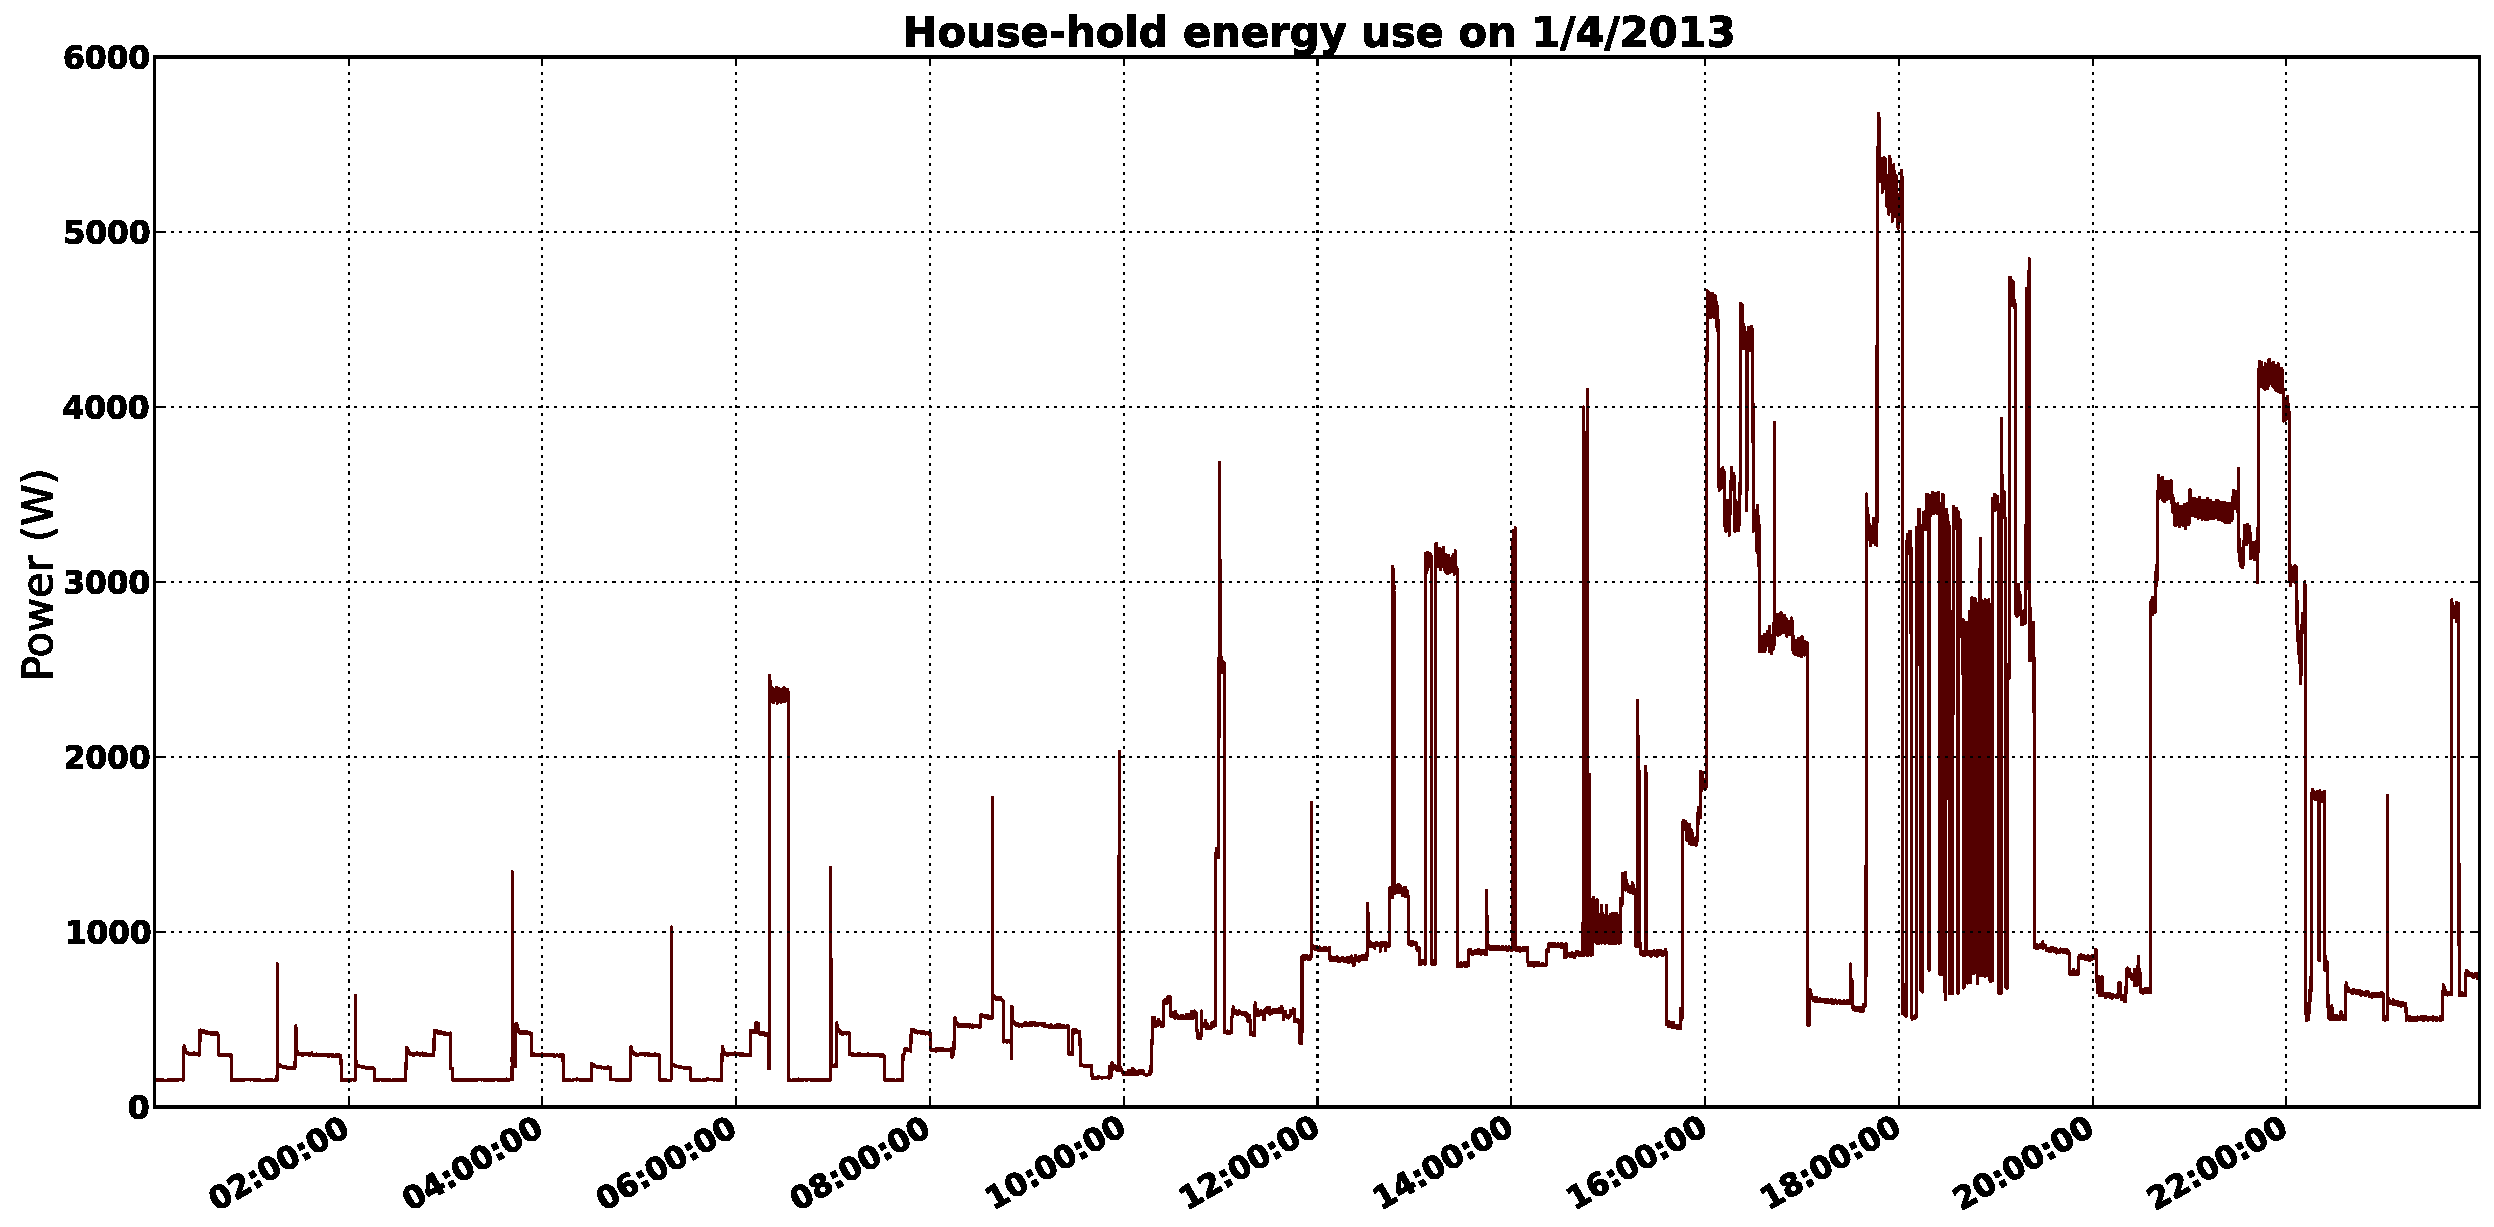
\includegraphics[width=14cm]{./notebooks/125_years_of_data_files/125_years_of_data_fig_04.pdf} 
\end{center}
}



\frame
{\frametitle{Profiling over ~5 months of data}
\begin{center}
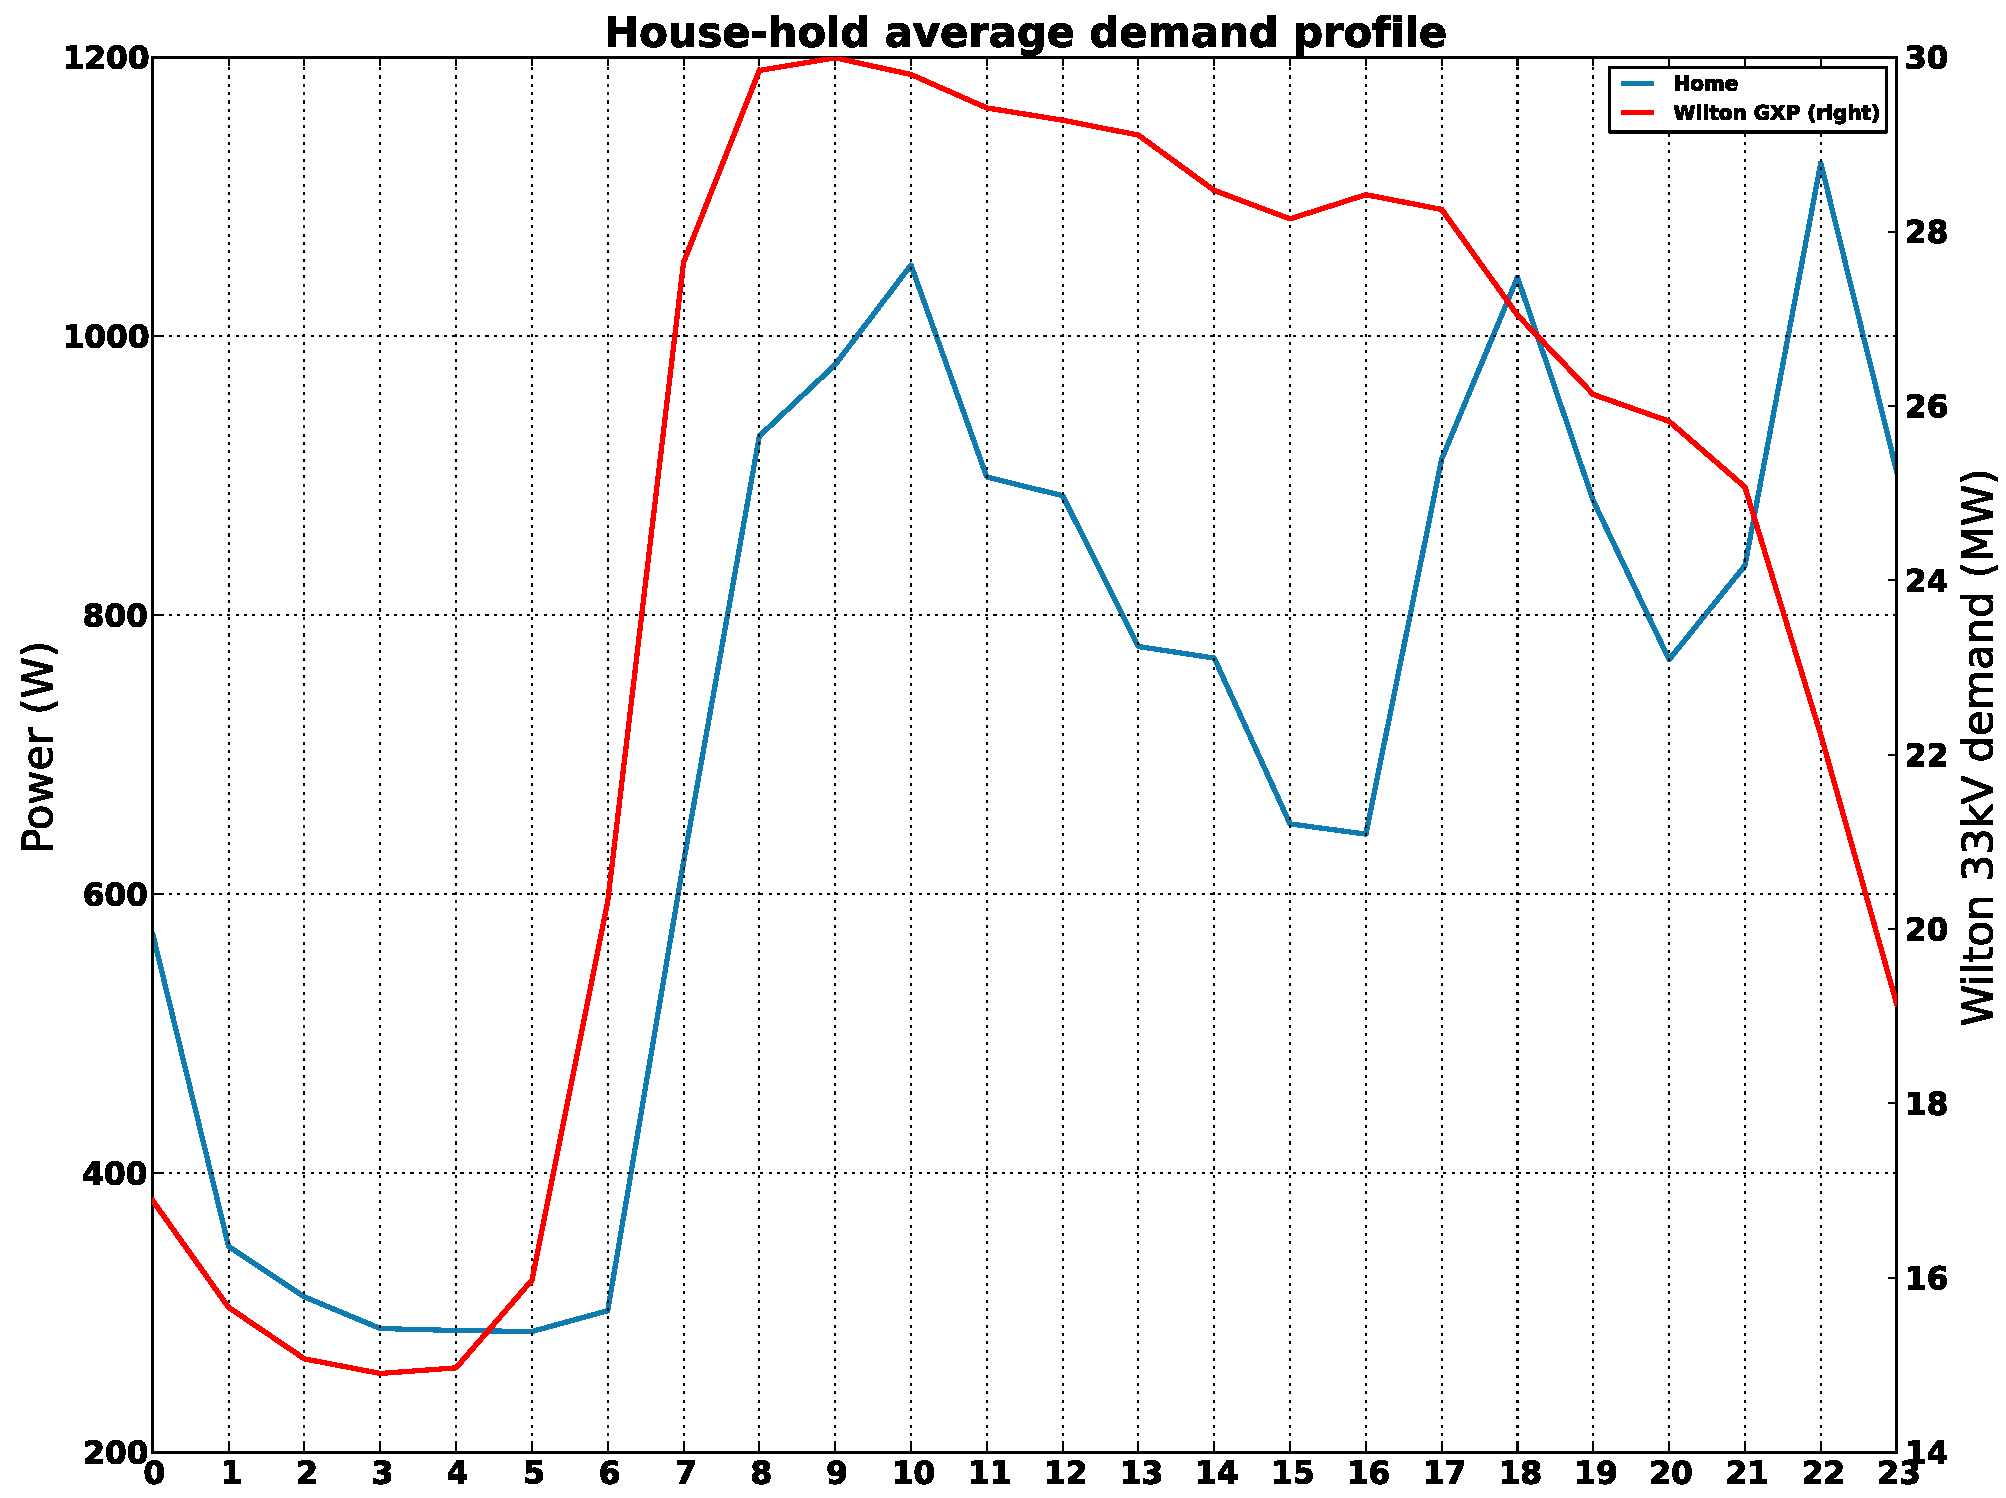
\includegraphics[width=9.5cm]{./notebooks/125_years_of_data_files/125_years_of_data_fig_05.pdf} 
\end{center}
}
\frame
{\frametitle{Bullendale -- 127 years ago}
\begin{columns}[t]
  \column[T]{3cm}
      \includegraphics[height=7.0cm]{bullendale3.png} 
  \column[T]{7cm}
  \vspace{5mm}
  \includegraphics[height=6.0cm]{bullendale1.png} 
\end{columns}
\begin{flushright}
\tiny \emph{Source: People, Politics and Power Stations}
\end{flushright}

}

\frame
{\frametitle{Bullendale -- 1986}
\begin{center}
\includegraphics[height=7.0cm]{bullendale2.png} 
\end{center}
\begin{flushright}
\tiny \emph{Source: Gold and electricity. Archaeological survey of Bullendale, Otago
}
\end{flushright}

}


\frame
{\frametitle{Reefton -- 125 years ago}
\begin{center}
\includegraphics[height=7.0cm]{reefton1.png} 
\end{center}
\begin{flushright}
\tiny \emph{Source: People, Politics and Power Stations}
\end{flushright}

}

\frame
{\frametitle{Reefton -- 125 years ago}
\begin{columns}[t]
  \column[T]{6cm}
   \includegraphics[height=6.0cm]{reefton2.png} 
  \column[T]{4cm}
  \vspace{5mm}
  \small Crompton DC bipolar dynamo
   \includegraphics[height=5.0cm]{reefton3.png} 
\end{columns}
\begin{flushright}
\tiny \emph{Source: People, Politics and Power Stations}
\end{flushright}

}

\frame
{\frametitle{Reefton -- today}
\begin{center}
\includegraphics[height=7.0cm]{reefton4.jpg} 
\end{center}
\begin{flushright}
\tiny \emph{Source: Wikipedia}
\end{flushright}
}



\frame
{\frametitle{EA Data Warehouse -- today}
\begin{center}
\includegraphics[width=11cm]{DW.png} 
\end{center}
}

\frame
{\frametitle{What about historic data\ldots}
\begin{columns}[t]
  \column[T]{5cm}
\includegraphics[height=7.5cm]{ppps.png} 
  \column[T]{5cm}
  \vspace{5mm}
  \includegraphics[width=5.0cm]{c_the_c.jpg}
\end{columns}
}

\begin{frame}[fragile]
  \frametitle{Historic data, NominalGenerationCapacity.txt (CDS)}
  \scriptsize
  \begin{verbatim}
Step Time,+-Difference
Nominal.Hydro.Bullendale                       Head 185' First industrial supply in N.Z. that left the building. For the quartz stamping battery via the first (low voltage) DC link.
   3/2/1886      50 Trial run. Two 50HP Pelton wheels drove two DC generators, 750RPM.
     1/1887       0 Breakdown.
     6/1887      60 I'll guess just a few months. Solid aron armatures replaced by laminated, so I'll allow for more oomph..
       1907       . Mined out.

Nominal.Hydro.Reefton                          Head 27' Reefton: first public supply in N.Z.
   1/8/1888@7pm  20 First demonstration of the first power station in N.Z. for the purposes of public supply. 30 and 110V DC Crompton dynamo.
       1901      46 New 220V Fynn dynamo, part-driven by an added steam engine salvaged from a wreck at Greymouth.
       1908      80 A 110HP Boving horizontal turbine replaced the 70HP Rafel turbine.
       1911       0 Power house destroyed by fire!
       1911     100 230V DC Lawrence Scott dynamo.
       1949     .   Reefton was connected to the national grid.
Nominal.Thermal.Reefton                        Steam power to support the Reefton hydro power scheme.
       1901      16 Guessed capacity of the auxiliary steam engine. A second boiler in 1920 (?) Inspection had shown 208V at the power house, 134V at the far end of distribution.
       1920      75 GEC dynamo. a 25HP Davey Paxman horizontal engine, a 20HP Marshall horizontal engine.
       1949       . In 1930 a standby diesel engine. Details lacking!

Nominal.Hydro.Wellington.PanamaStreet          Head ~100'? Water main supply, discharge to the harbour..
     6/1889      30 Water mains supplied (at no charge) two 30HP "vortex" turbines driving a 15KW Gulcher single phase AC generator at 100V and 80cps. What happened to the extra HP?
       1891    +110 Three 50HP turbines driving five generators were installed on the closure of the Manners Street station

  \end{verbatim}
\end{frame}


\frame
{\frametitle{Historic data example -- Cobb}
\begin{center}
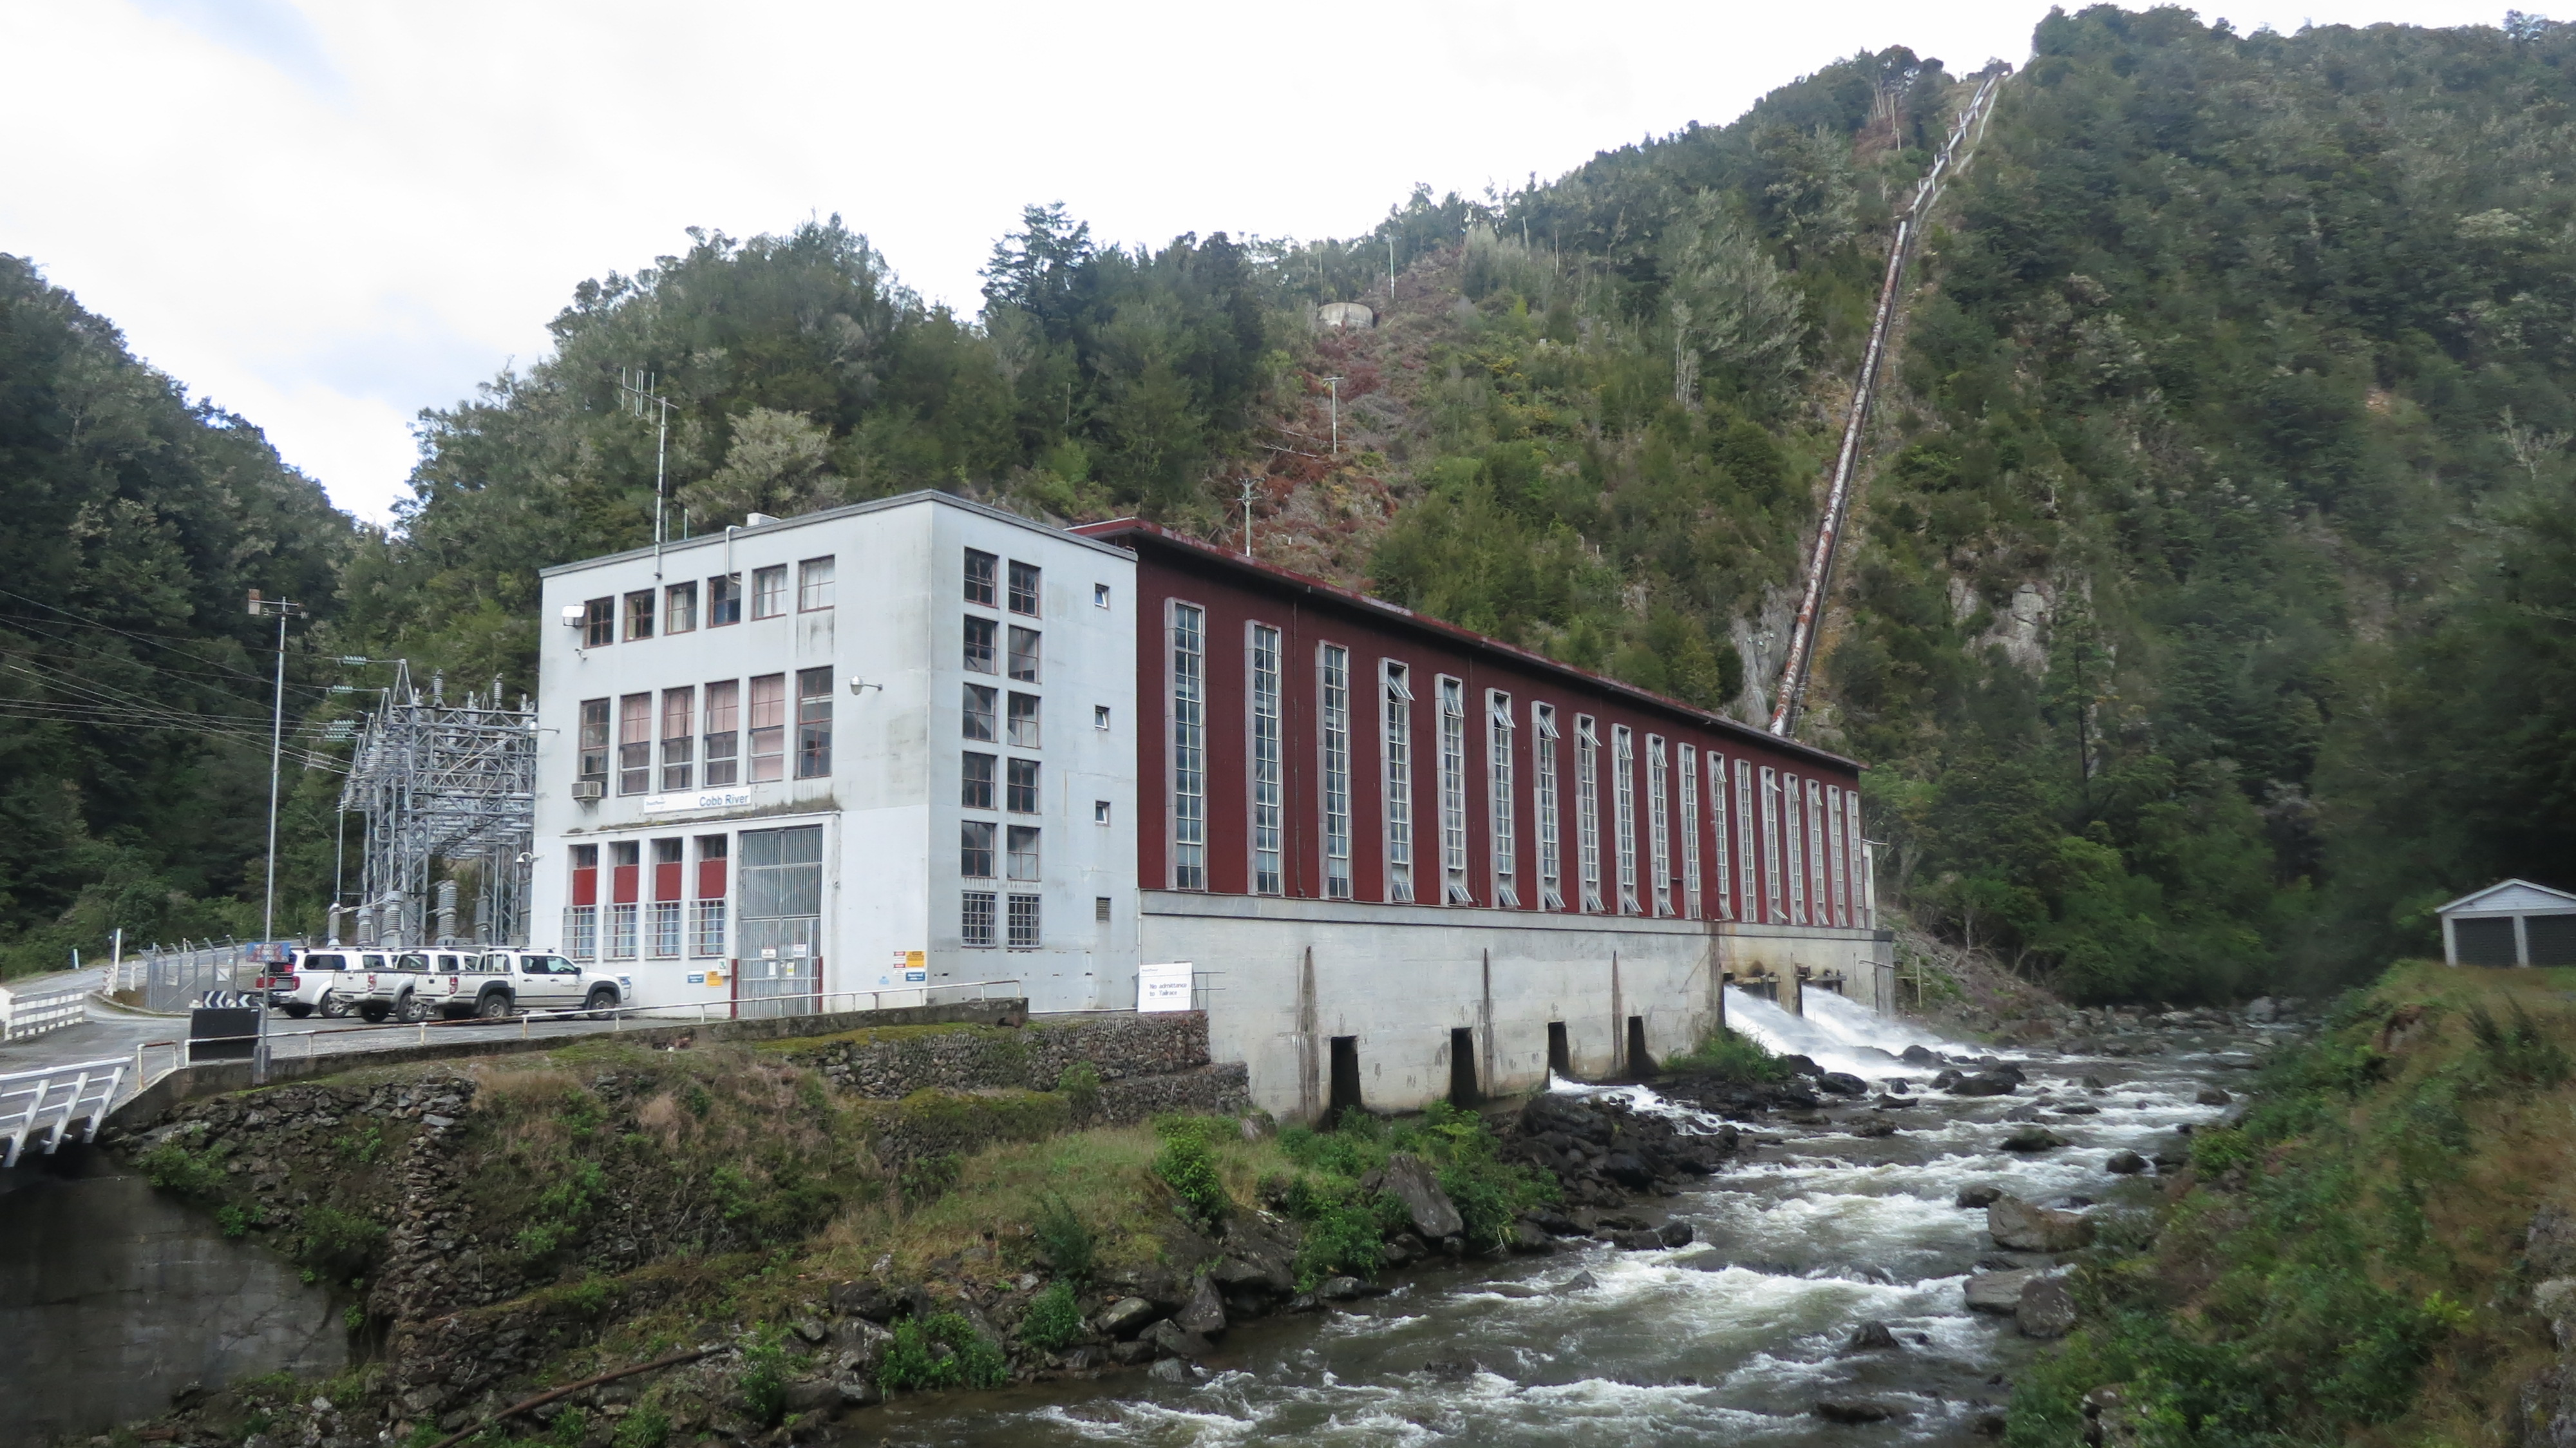
\includegraphics[height=7.5cm]{cobb.jpg} 
\end{center}
}


\begin{frame}[fragile]
  \frametitle{Historic data, NominalGenerationCapacity.txt (CDS)}
  \vspace{-0.5mm}
  \scriptsize
  \begin{verbatim}
Nominal.Hydro.Cobb                             Head 1876' then 1950' after the earth dam of 107' replaced the weir and its ad-hoc extensions. Highest head in N.Z. with the water jet emerging at about a third of the speed of sound.
 23/ 5/1944@3pm       3000 Trial generation, supplied to the Golden Bay Power Board via Motupipi substation. The power house had been completed in 1938, with the generators waiting in wrappings.
 28/ 5/1944@4:40pm    9000 Three generators working. First transmission to the Stoke substation.
 14/ 6/1944@1pm      12000 Four 3MW single-jet pelton wheels. Ceremony in the afternoon, with Cobb taking over from the Stoke diesel plant. Prices dropped to one penny per KWh.
 17/12/1949@11pm         0 Old intake tunnel closed, as it was in the way of the new dam's spillway intake.
 18/12/1949@5pm      12000 Temporary intake connected to the long tunnel through the hill.
        1950         13000 Run on overload.
      1/1953         10000 Summer water shortage, again. Lake Cobb's exit had been blasted open, and Lake Sylvester sucked down to sludge.
      3/1954         13000 A March deluge! Full power, then.
  19/ 9/1954@6:20pm  10000 New penstock and generators start, the old overhauled. Two 10MW double-jet pelton wheels in an expanded powerhouse. An earth dam forming lake Cobb replaced the weir (with optional added sandbags).
  20/ 9/1954@5:15pm +10000 Second new generator started.
      2/1955         16000 Lack of water forced a 20% cut.
      3/1955         32000 Another March deluge, but this time less fear of overtopping the dam under construction.
      4/1955         25000 Run out of water already!
      5/1955         32000 Some filling allowed, the lower lake backing to Lake Halley. The desperate need for power outran the ability to remove buildings before they were drowned! Final filling in October,
  26/ 1/1968             0 Harry's mistake! Generator 1 was under maintenance, and the water valve was opened. The jet blasted through the powerhouse wall, wrecked the transformer yard and deflected from the cliff behind flew across the road to splinter two trees on the far side of the river.
  27/ 1/1968@9:30pm  20000 Generators 5 and 6 back in service after much scrabbling. I'll guess that these are the two 10MW generators.
      2/1968         32000 I'll guess all are back.
      1/1975             0 Drought. Shutdown to keep silt out of the works!
      3/1975         32000 I'll guess that March again refilled the lake.
  16/11/1981@1:09am      0 Landslide! Carried away a section of both pipelines.
  19/ 8/1982         20000 First two generators activated. All had absorbed moisture in the cool powerhouse...
  20/ 8/1982         32000 Full power.

  \end{verbatim}
\end{frame}

%\frame
%{\frametitle{Historic data, NominalGenerationCapacity.txt (CDS)}
%\begin{center}
%\includegraphics[height=6.0cm]{NominalGenerationCapacity_COB.png} 
%\end{center}
%}



\frame
{\frametitle{Nameplate generation growth}
\begin{center}
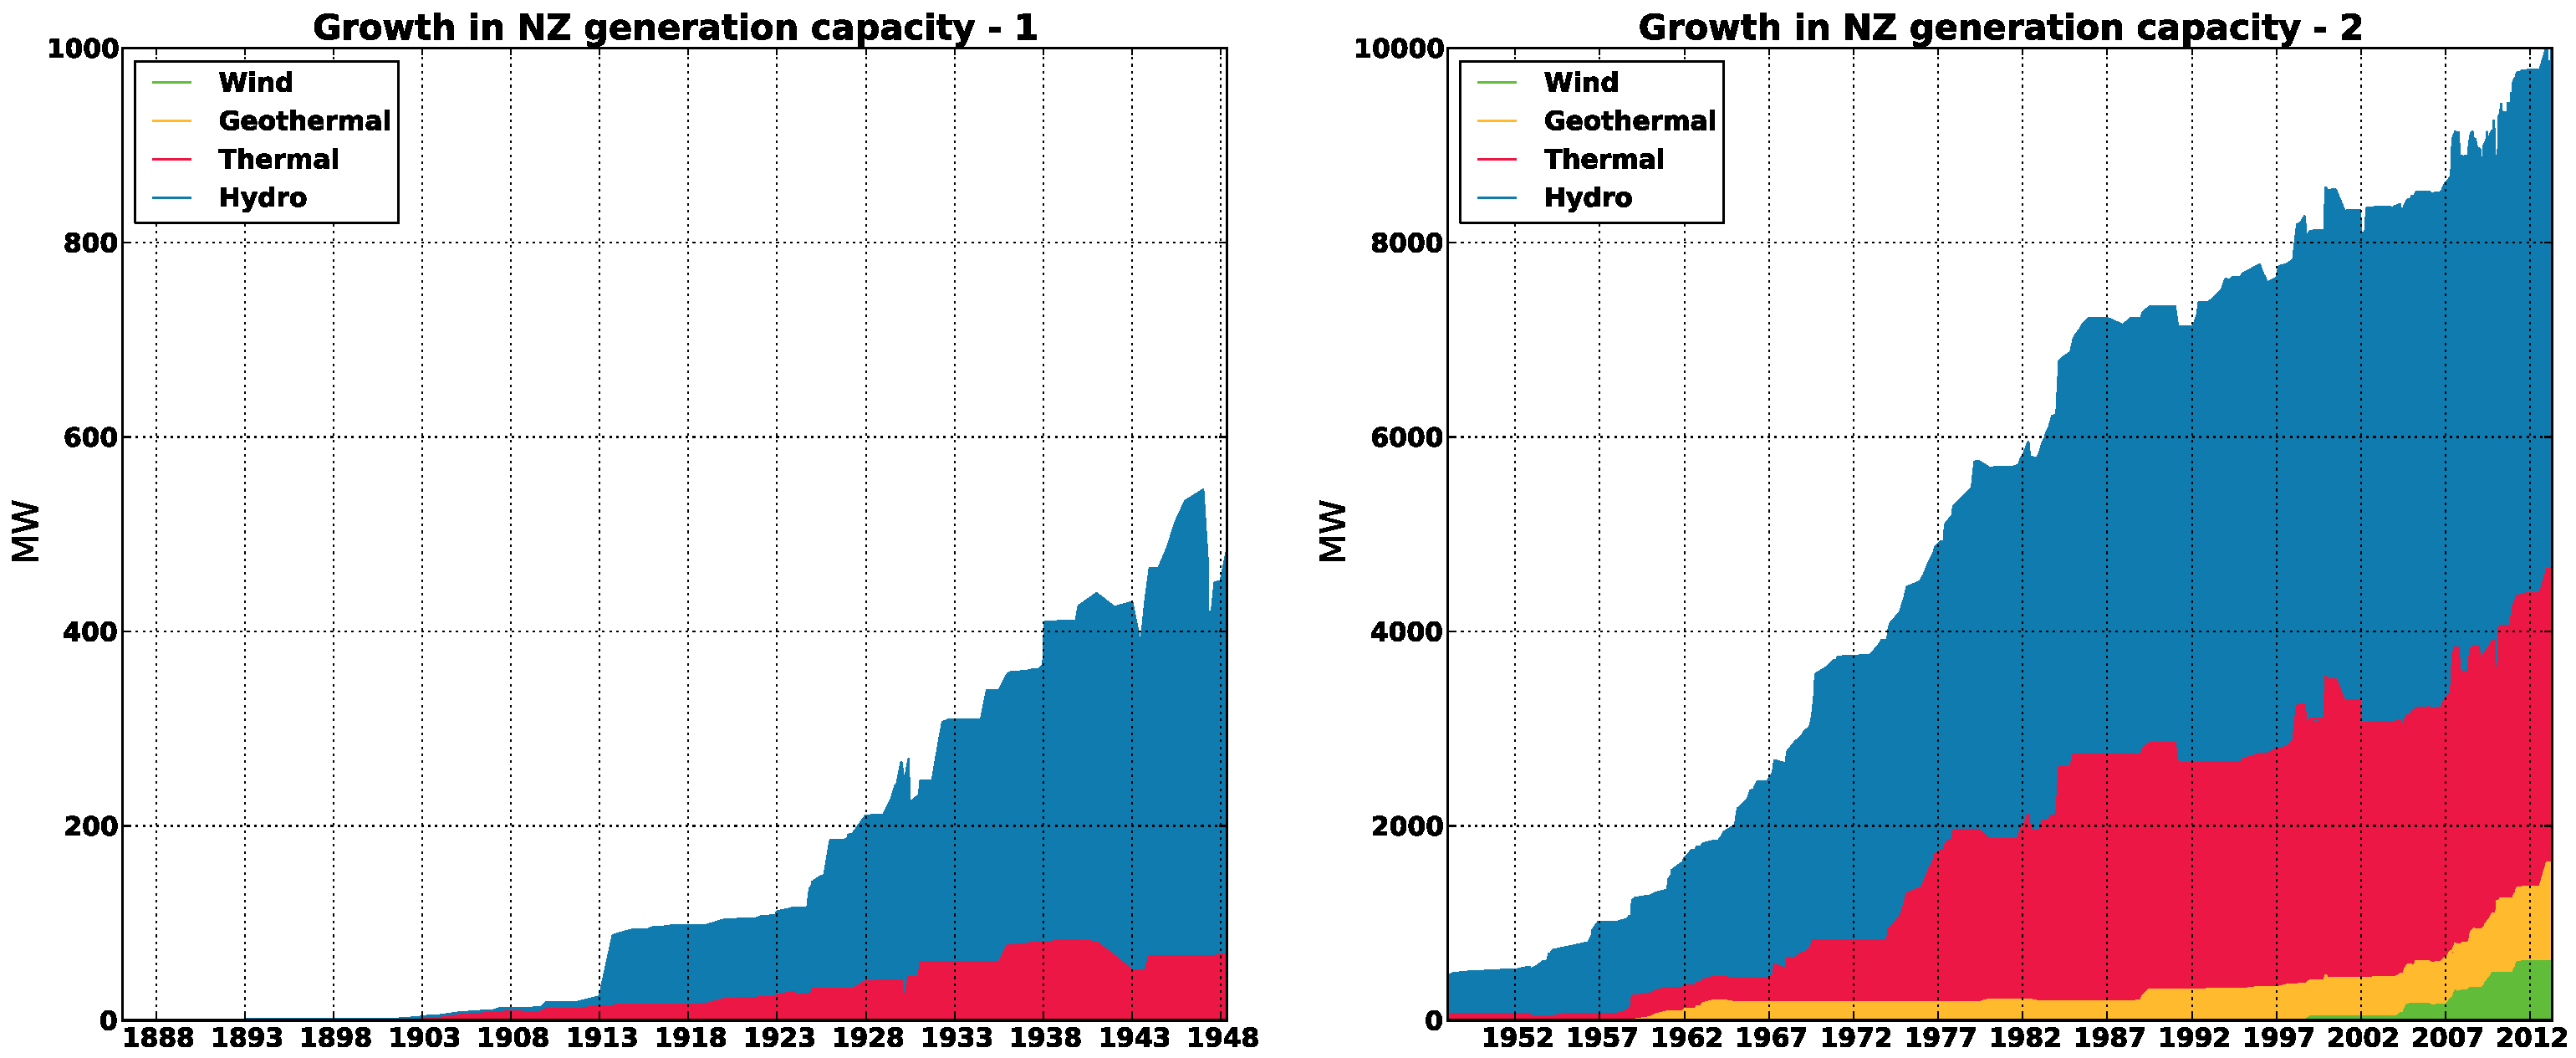
\includegraphics[width=14cm]{./notebooks/125_years_of_data_files/125_years_of_data_fig_00.pdf} 
\end{center}
}

%This is a picture of the outback inverter and battery bank

%\frame
%{\frametitle{Last 20 years...}
%\begin{center}
%\includegraphics[width=7cm]%{./notebooks/125_years_of_data_files/125_years_of_data_fig_01.pdf} 
%\end{center}
%}

%This is a picture of the GB Weekly ad for "Power cut" Sunday

\frame
{\frametitle{\% growth by generation type}
\begin{center}
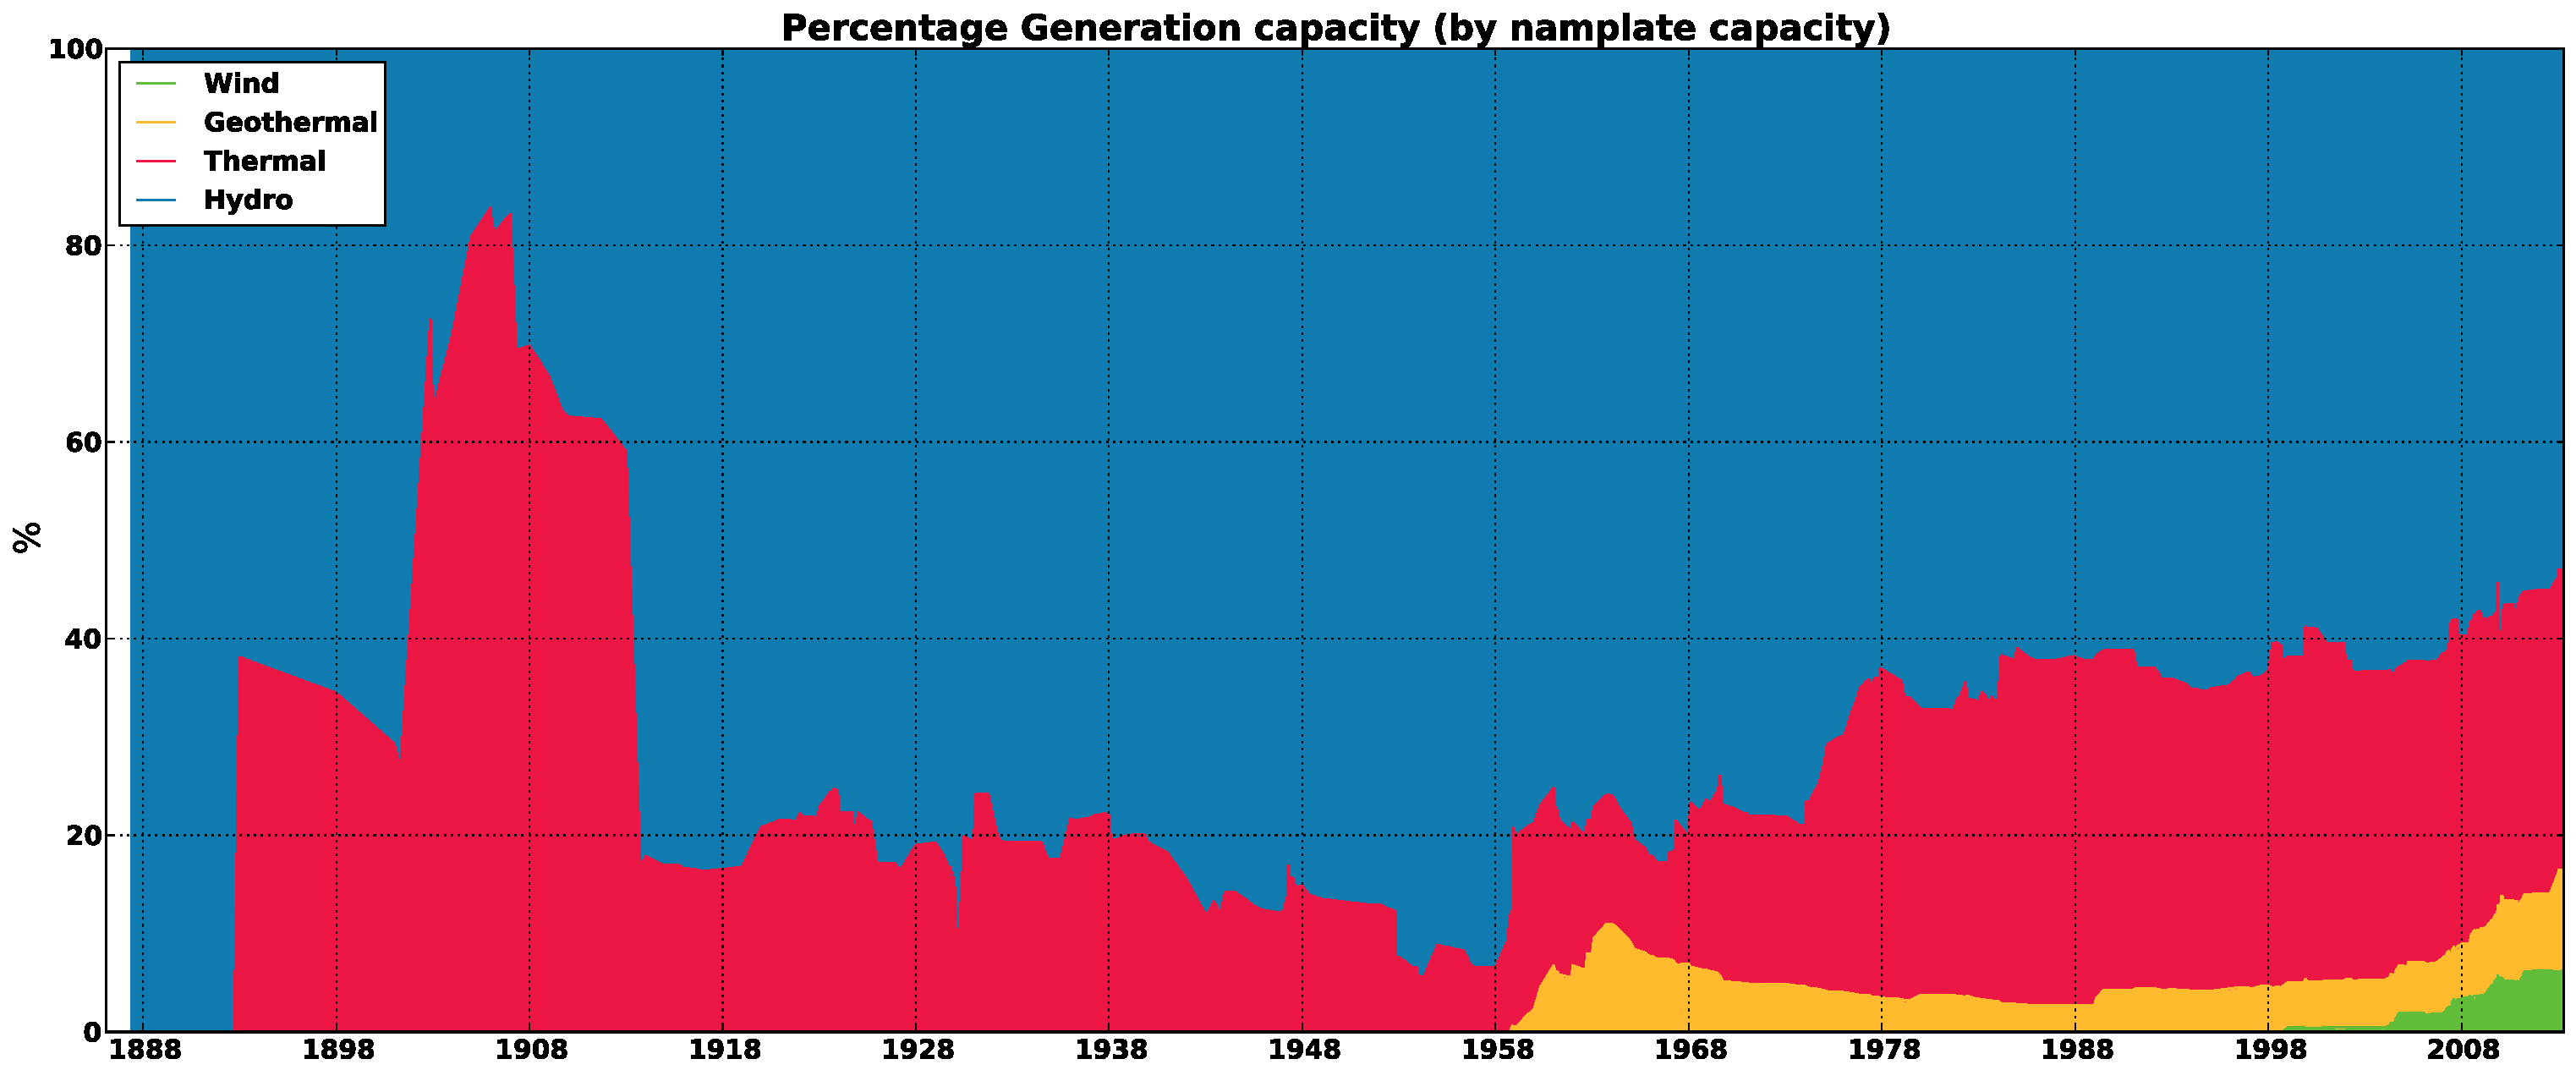
\includegraphics[width=14cm]{./notebooks/125_years_of_data_files/125_years_of_data_fig_02.pdf} 
\end{center}
}

%\frame
%{\frametitle{A few insteresting historic events}
%\begin{center}
%\includegraphics[width=15cm]{NominalGenerationCapacity_COB.png} 
%\end{center}

%}

\begin{frame}[fragile]
  \frametitle{Insteresting historic generation events}
  \scriptsize
  \begin{verbatim}
Nominal.Hydro.Reefton                          Head 27' Reefton: first public supply in N.Z.
       1911       0 Power house destroyed by fire!
Nominal.Hydro.Kourarau                         Two power stations and pipes not shown on the topographic maps.
    12/1924       0 Power house drowned by a flood!
     4/2005    -700 Station A again flooded.
     8/2006       0 Cracks in the upper station's penstock, water coming down the hillside...
Nominal.Hydro.Waikato.Arapuni                  Head 175'
   4/6/1929   15000 Early start before the power house was finished, Auckland being needy.
   7/6/1930       0 Seepage. Leakage. Cracks! Voids! Ground movement! EMERGENCY! Criticism! Censorship! Denials! Desperate recourse to all other available generation!
Nominal.Hydro.DawsonFalls                      Head 220' Dawson Falls Lodge. Mains electricity arrived in 1982.
  21/2/1935       0 Flood!
Nominal.Hydro.Matahina                         Head 200'
     2/1967       0 Leakage discovered, subsidence...
    12/1987       0 Decomissioned in December for repairs after the Edgecumbe earthquake of the second of March.
Nominal.Hydro.Cobb                             Head 1876' then 1950' after the earth dam of 107' replaced the weir and its ad-hoc extensions. Highest head in N.Z. with the water jet emerging at about a third of the speed of sound.
  26/ 1/1968             0 Harry's mistake! Generator 1 was under maintenance, and the water valve was opened. The jet blasted through the powerhouse wall, wrecked the transformer yard and deflected from the cliff behind flew across the road to splinter two trees on the far side of the river.
  16/11/1981@1:09am      0 Landslide! Carried away a section of both pipelines.
Nominal.Hydro.Kaniere.KaniereForks             Head ~250' Conversion of goldminer's works.
       1973       0 Collapse of the Johnson's flume.
     6/1979       0 Fire! The generators had to be rewound. A rat chewing at cables was suspected.
     6/1981       0 Fire again!! This time the machines had overheated.
Nominal.Hydro.Ruahihi                          Head 280' Canal from Lake McLaren, superceding the McLaren Falls power station.
  20/9/1981@1:50pm . Canal failure! Wipeout!
  \end{verbatim}
\end{frame}


\frame
{\frametitle{April 1947}
\begin{center}
\includegraphics[height=7.0cm]{horahora.png} 
\end{center}
\begin{flushright}
\tiny \emph{Source: People, Politics and Power Stations}
\end{flushright}

}


\begin{frame}[fragile]
  \frametitle{Insteresting historic generation events}
  \scriptsize
  \begin{verbatim}
Nominal.Hydro.Pupu                             Head 300' Conversion of a goldminer's water race.
       1981       . A "flashover" ruined the generator.
Nominal.Hydro.Wheao                            Head ~400' Downcanal of Flaxy.
       1983   24000 Two turbines. Destroyed by canal failure just before completion, 30'th December 1982.
Nominal.Hydro.OmanawaFalls                     Head 100' Underground power house.
     4/1985       0 Cotton insulation on the winding failed! I'll guess the months.
Nominal.Hydro.Glenorchy                        Head 210' Pipeline from the Ox Burn dam.
     1/1994       0 Very heavy rain caused floods and landslides. Detritus reached the roofline of the powerhouse.
Nominal.Hydro.Tokaanu                          Head 682'
       1996  240000 Volcanic ash from the 1995 Mount Ruapehu eruption damaged the turbines. Refurbished to 60MW.
Nominal.Hydro.Rangipo                          Head 788' Underground power house.
     4/1996       0 Ash from eruptions at Ruapehu badly damaged the turbines
Nominal.Hydro.RoaringMeg.Lower                 Head 1000'
    11/1999       0 Flood! The control equipment was ruined.
Nominal.Hydro.Opuha                            Head 160' Overwhelmed by a flood during construction, 6'th Feb 1997. Assorted excitements follow. River flow restrictions usually limit full-power generation to bursts of a few hours at a go.
 13/01/2001       0 The washout weir washed out.
    11/2003       0 Fire destroyed the generators! Or possibly in 2005.
 17/05/2009@6:10  0 Another washout.
Nominal.Wind.GebbiesPass                       Wind turbine, test installation.
  10/3/2005       0 Wrenched apart by wind swirl!
Nominal.Hydro.Karaponga                        Head ~30 feet. Guesswork: the dam is 18'5"
     9/2010       0 Penstocks imploded!

  \end{verbatim}
\end{frame}


\frame
{\frametitle{22 October 1968}
\begin{center}
\includegraphics[height=7.0cm]{manapouri.jpg} 
\end{center}
\begin{flushright}
\tiny \emph{Source: \url{http://www.flickr.com/photos/sharman/6690836457/}}
\end{flushright}

}



\begin{frame}[fragile]
  \frametitle{What about Transmission? Unplanned Outage Data (CDS)}
  \begin{verbatim}
        Ident   Flt_Item Rem_Item Start             End  \                                            
        SS99101 LIV-NSY1 LIV-NSY1 1999-07-02 11:20 1999-07-02 11:30   
                         NSY-TF-1 1999-07-02 11:20 1999-07-02 11:40   
                         NSY-TF-2 1999-07-02 11:20 1999-07-02 11:41   
                         NSY-ROX1 1999-07-02 11:20 1999-07-02 11:30   
        SS99102 CML-FKN2 CML-FKN2 1999-07-02 22:13 1999-07-02 22:36   
                         FKN-TF-4 1999-07-02 22:13 1999-07-02 22:38   
        SS99103 CML-FKN2 CML-FKN2 1999-07-02 22:50 1999-07-02 23:00   
                         FKN-TF-4 1999-07-02 22:50 1999-07-02 23:16   
        SS99104 CML-FKN1 CML-FKN1 1999-07-02 23:04 1999-07-02 23:11   
                         FKN-TF-2 1999-07-02 23:04 1999-07-02 23:12   
        SS99105 CML-FKN2 CML-FKN2 1999-07-02 23:09 1999-07-03 16:27   
                         FKN-TF-4 1999-07-02 23:09 1999-07-03 16:27   

  \end{verbatim}

 % \begin{itemize}
 %   \item First point about slab of verbatim
 %   \item Isn't verbatim great?
 % \end{itemize}
\end{frame}

\frame
{\frametitle{Transmission annual forced outage counts}
\begin{center}
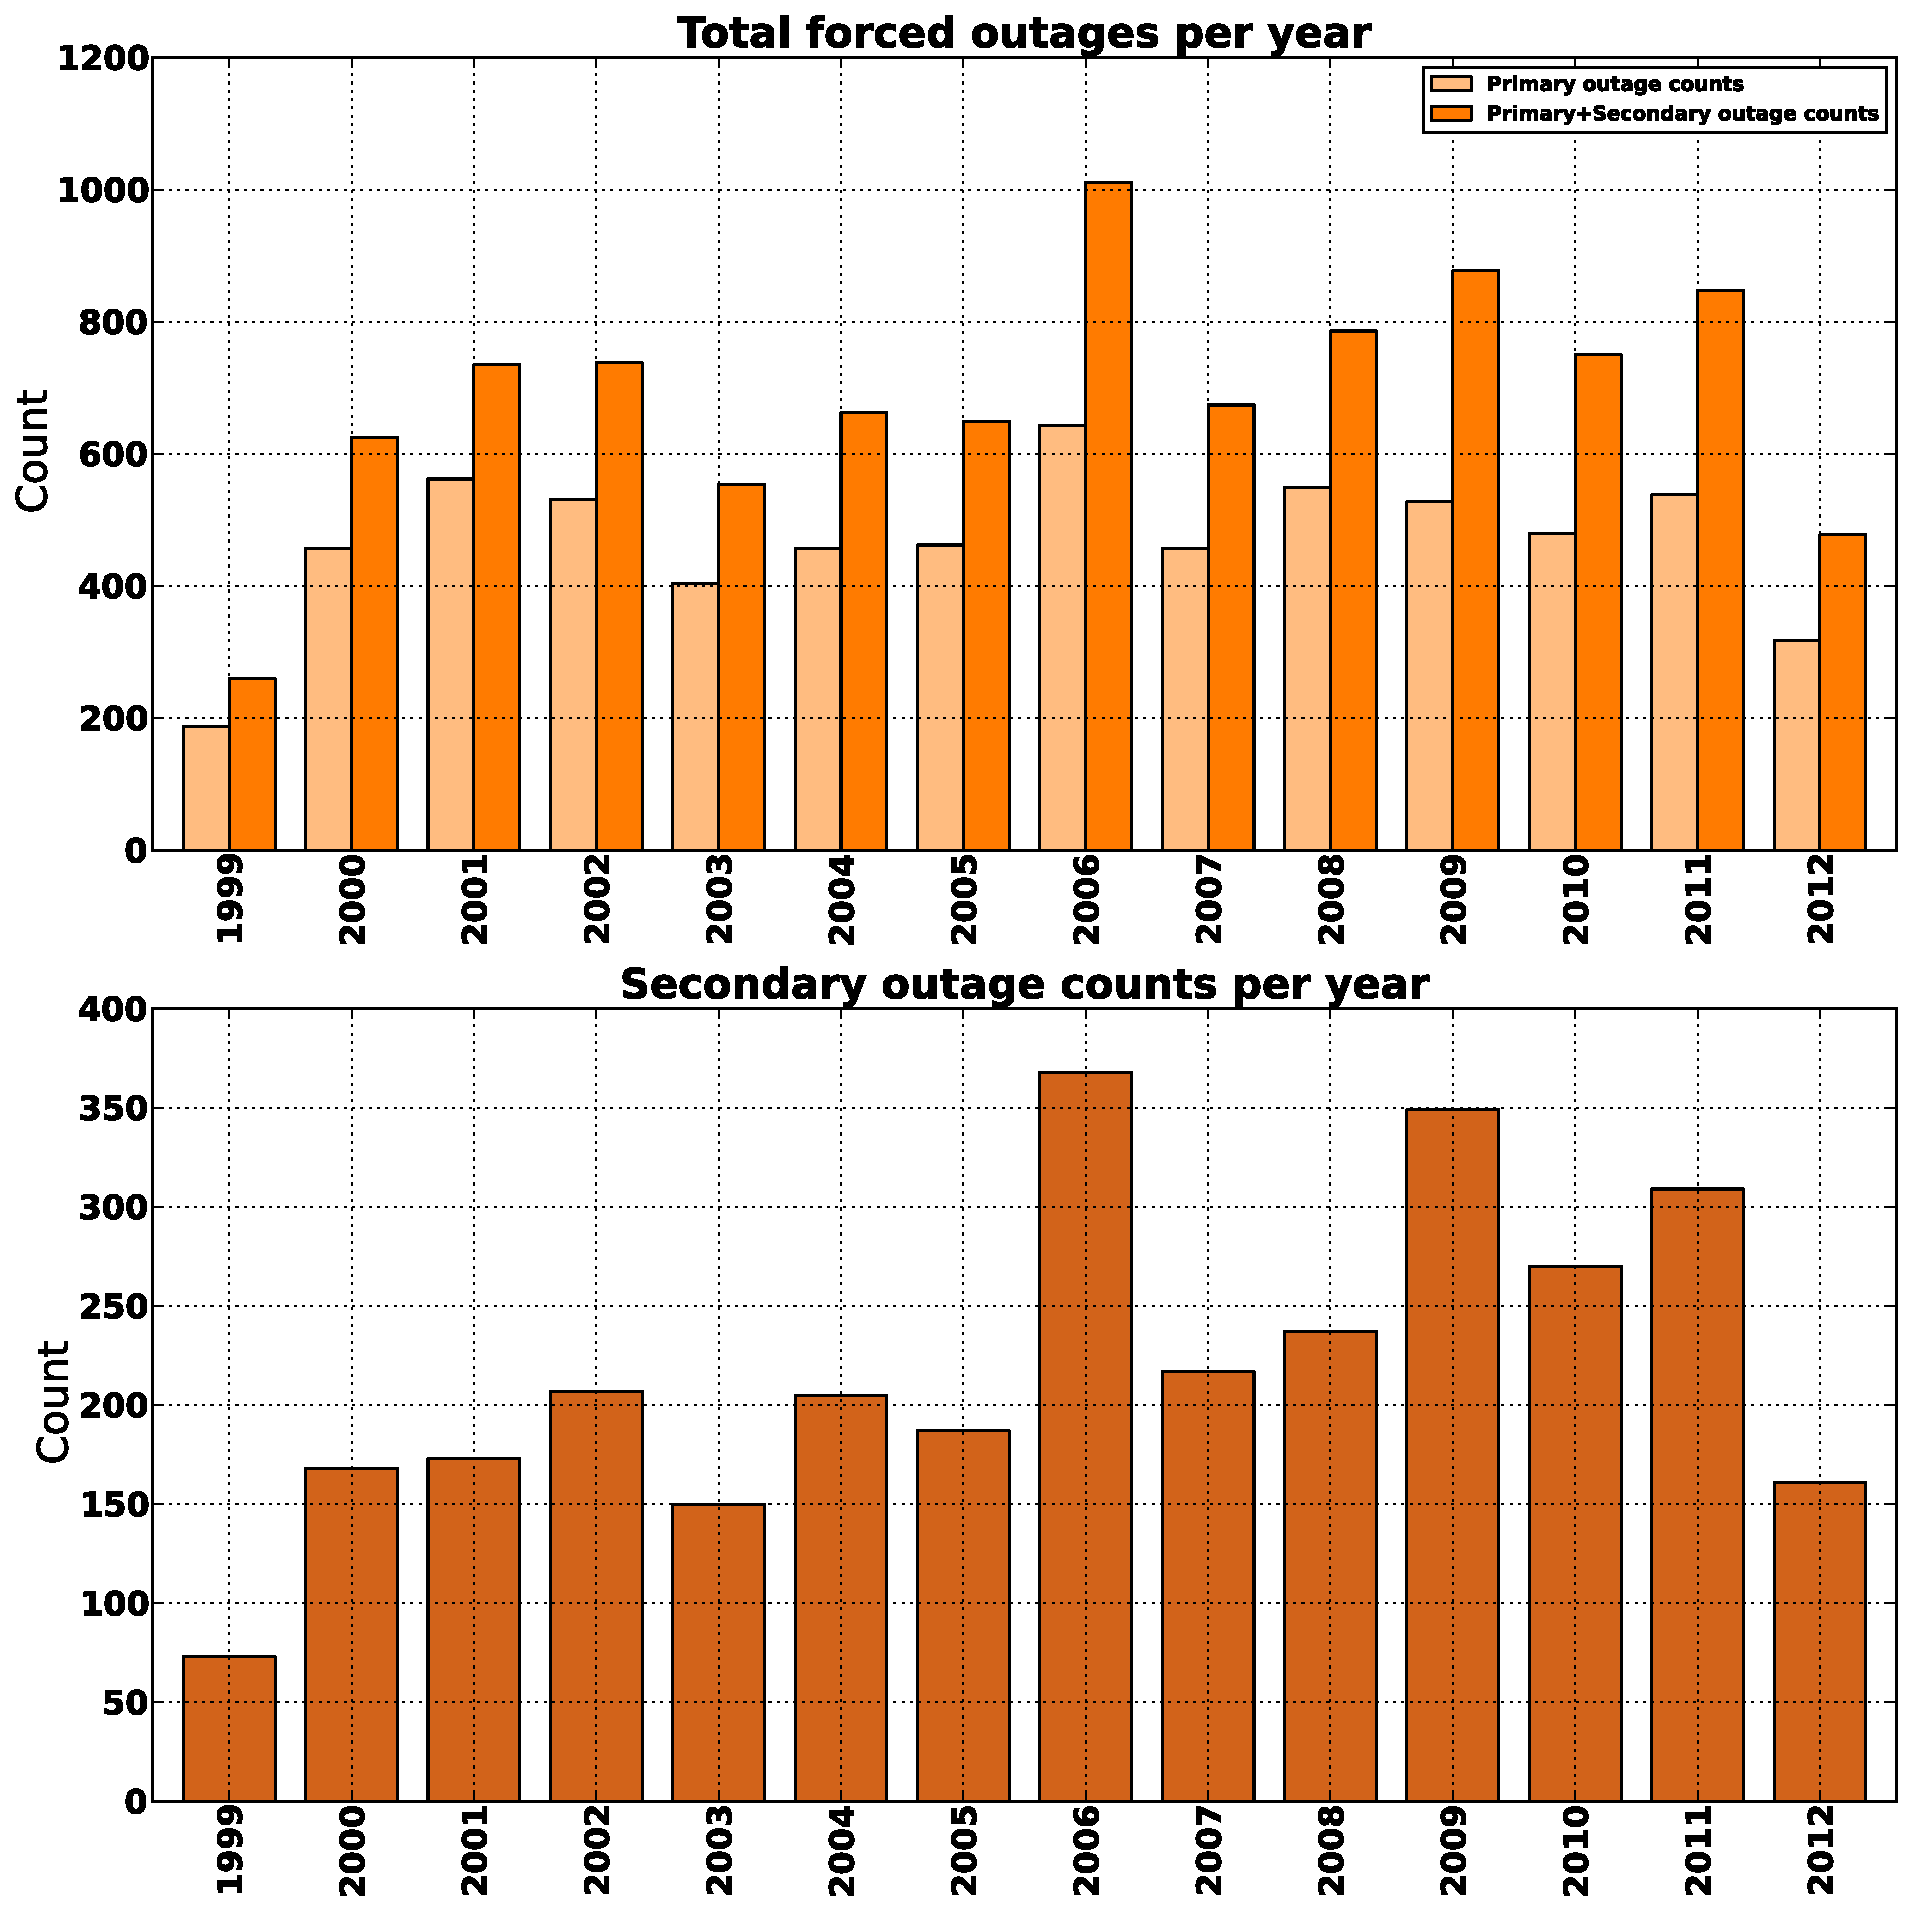
\includegraphics[width=7.5cm]{./notebooks/125_years_of_data_files/125_years_of_data_fig_07.pdf} 
\end{center}
}

\frame
{\frametitle{Transmission -- primary fault trend}
\begin{center}
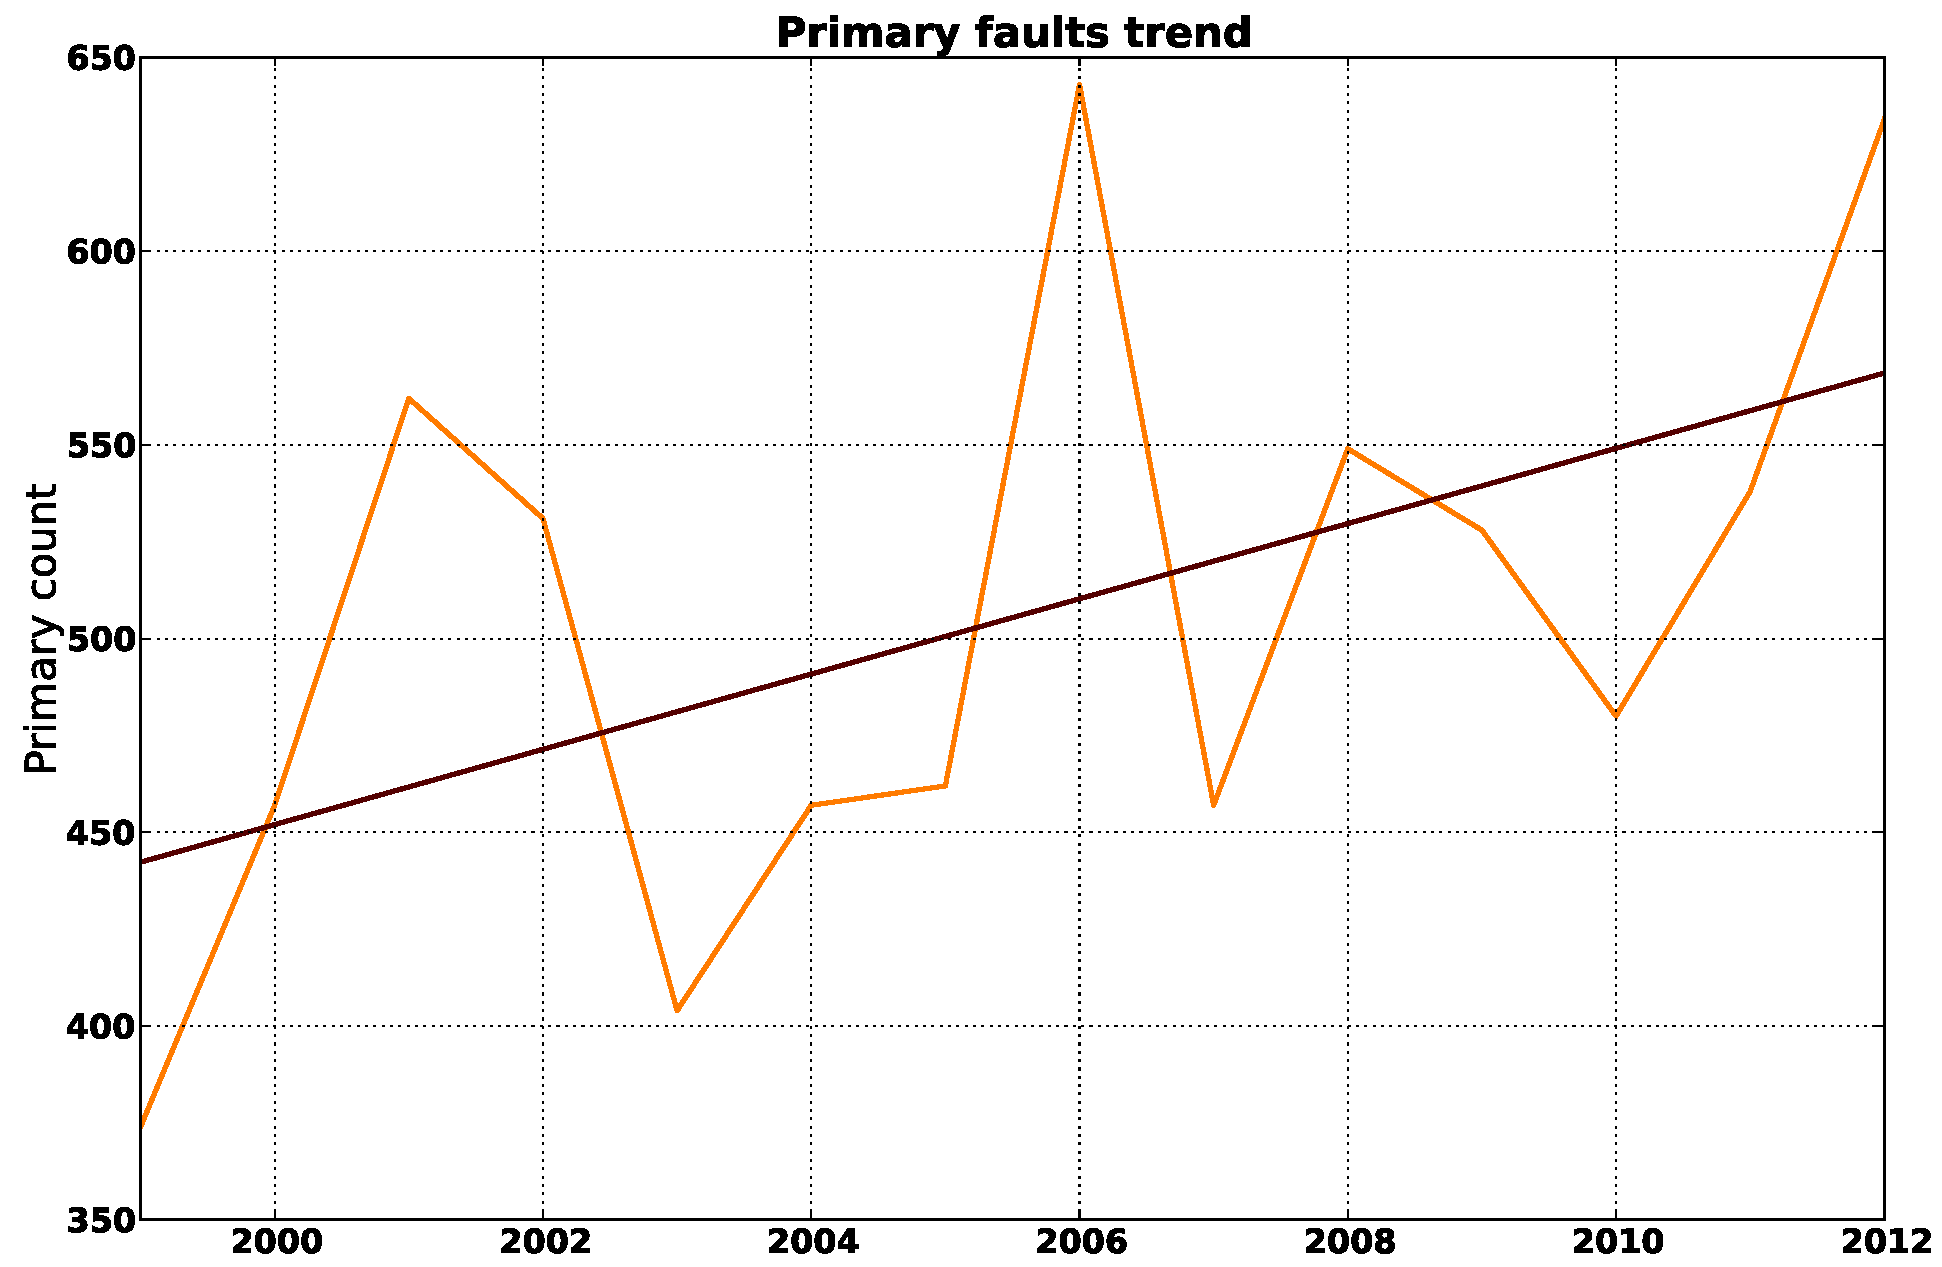
\includegraphics[width=11cm]{./notebooks/125_years_of_data_files/125_years_of_data_fig_08.pdf} 
\end{center}
}

\begin{frame}[fragile]
  \frametitle{Transmission -- Primary fault trend - OLS regression results}
\scriptsize
\begin{verbatim}
                                    OLS Regression Results                            
        ==============================================================================
        Dep. Variable:                 counts   R-squared:                       0.268
        Model:                            OLS   Adj. R-squared:                  0.207
        Method:                 Least Squares   F-statistic:                     4.403
        Date:                Thu, 11 Apr 2013   Prob (F-statistic):             0.0577
        Time:                        12:45:40   Log-Likelihood:                -78.224
        No. Observations:                  14   AIC:                             160.4
        Df Residuals:                      12   BIC:                             161.7
        Df Model:                           1                                         
        ==============================================================================
                         coef    std err          t      P>|t|      [95.0% Conf. Int.]
        ------------------------------------------------------------------------------
        const        442.3143     35.394     12.497      0.000       365.198   519.431
        index          9.7099      4.628      2.098      0.058        -0.373    19.792
        ==============================================================================
        Omnibus:                        1.625   Durbin-Watson:                   2.141
        Prob(Omnibus):                  0.444   Jarque-Bera (JB):                1.281
        Skew:                           0.630   Prob(JB):                        0.527
        Kurtosis:                       2.220   Cond. No.                         14.7
        ==============================================================================
\end{verbatim}
\end{frame}

\begin{frame}[fragile]
  \frametitle{Transmission -- Primary fault trend -- OLS regression results}

\begin{itemize}
   \item[--] highly variable
   \item[--] results borderline 
   \item[--] can't conclusively state primary forced outage rate is growing 
   \item[--] what about annual secondary outage counts?}
\end{itemize}

\end{frame}

\frame
{\frametitle{Transmission -- Secondary fault trend}
\begin{center}
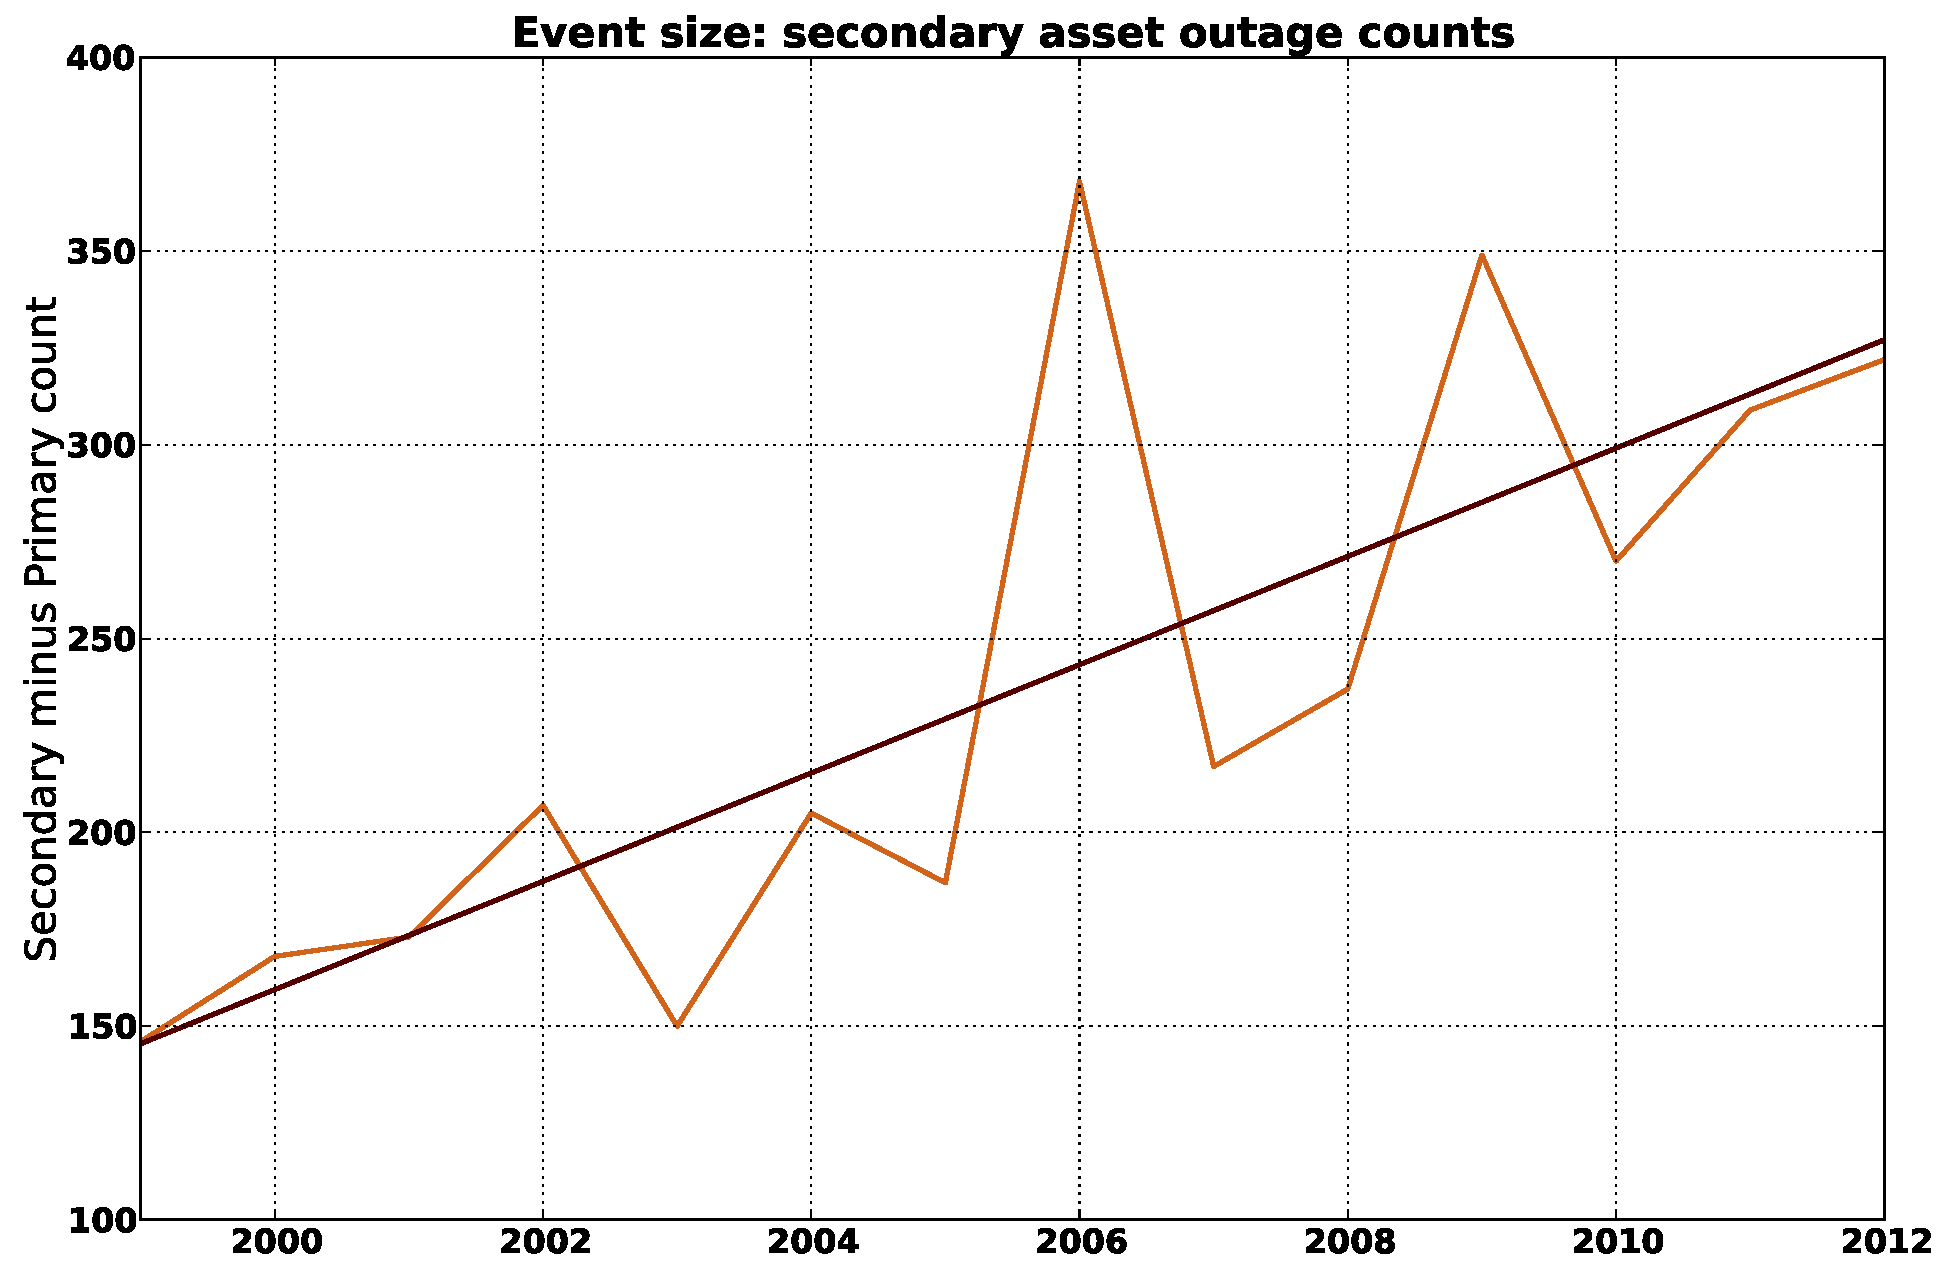
\includegraphics[width=11cm]{./notebooks/125_years_of_data_files/125_years_of_data_fig_09.pdf} 
\end{center}
}

\begin{frame}[fragile]
  \frametitle{Transmission -- Secondary fault trend - OLS regression results}
\scriptsize
\begin{verbatim}
                                     OLS Regression Results                            
        ==============================================================================
        Dep. Variable:                 counts   R-squared:                       0.611
        Model:                            OLS   Adj. R-squared:                  0.578
        Method:                 Least Squares   F-statistic:                     18.83
        Date:                Tue, 09 Apr 2013   Prob (F-statistic):           0.000962
        Time:                        12:01:37   Log-Likelihood:                -73.147
        No. Observations:                  14   AIC:                             150.3
        Df Residuals:                      12   BIC:                             151.6
        Df Model:                           1                                         
        ==============================================================================
                         coef    std err          t      P>|t|      [95.0% Conf. Int.]
        ------------------------------------------------------------------------------
        const        145.4571     24.628      5.906      0.000        91.798   199.117
        index         13.9736      3.220      4.340      0.001         6.958    20.989
        ==============================================================================
        Omnibus:                       11.111   Durbin-Watson:                   2.908
        Prob(Omnibus):                  0.004   Jarque-Bera (JB):                6.867
        Skew:                           1.466   Prob(JB):                       0.0323
        Kurtosis:                       4.782   Cond. No.                         14.7
        ==============================================================================
\end{verbatim}
\end{frame}

\begin{frame}[fragile]
  \frametitle{Transmission -- Secondary fault trend - OLS regression results}

\begin{itemize}
   \item[--] results more statistically conclusive 
   \item[--] size of transmission outages, in terms of secondary equipment, is on the increase
   \item[--] Average rate of growth $\approx$14 additional secondary outages/year, over past 13 years
   \item[--] 95\% confidence interval indicates between 7 and 21 additional outages per year
   \item[--] \textbf{Conclusion:} More secondary assets are being tripped?  \textbf{Why?} 
\end{itemize}
\end{frame}

%\begin{frame}[fragile]
%  \frametitle{}
%
%\begin{itemize}
%\item increased system size?;
%\item increased peak demand?;
%\item increased complexity (protection systems and settings?)
%\item increased human error?; 
%\item data/communication issues?
%\item actual reported dataset issues?
%\item lack of maintenance?; 
%\item lack of co-ordination in planned outages? 
%\end{itemize}
%\end{frame}

\begin{frame}[fragile]
  \frametitle{Real-time spot market monitoring}

\begin{itemize}
   \item[--] fully open source Python based system developed:
   \begin{itemize}
       \item[--] connects to the NZX WITS FTP server
       \item[--] attempts download of most recent real time price file 
       \item[--] prices parsed into memory, stored, statisics calculated, logged
       \item[--] if prices $>$ threshold, sends text alerts
       \item[--] prices graphed using Javascript/d3 (EA intranet)
       
   \end{itemize}
\end{itemize}

\end{frame}

\frame
{\frametitle{Real-time spot market monitoring, weekly time-series data}

Example: Weekly horizon charts, updated every 5 minutes (Hawkes Bay GXPs)
\begin{center}
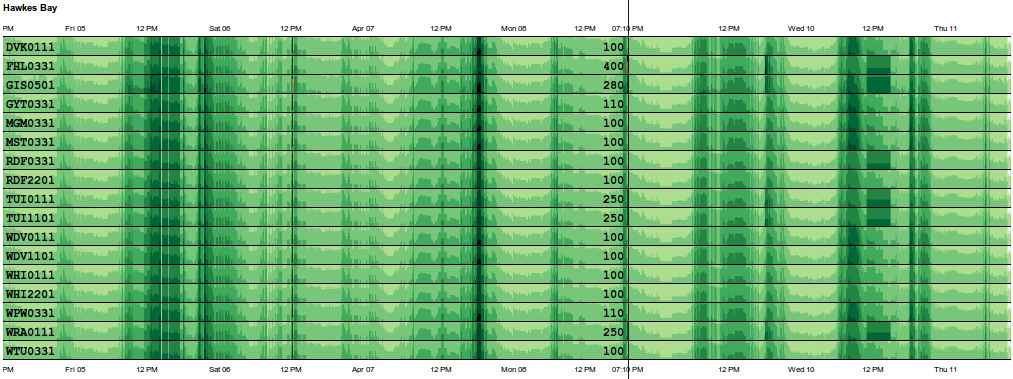
\includegraphics[width=14.5cm]{./notebooks/rtpm2.png} 
\end{center}
}


\frame
{\frametitle{Real-time spot market monitoring, NZ jigsaw (Choropleth)}
\begin{columns}[t]
  \column[T]{5cm}
     \includegraphics[height=7.5cm]{./nz_price.png} 
  \column[T]{5cm}
  \vspace{0mm}
     \includegraphics[height=7.5cm]{./nz_price_2.png} 
\end{columns}
\begin{tikzpicture}[remember picture,overlay]
\node (feb22) [xshift=5.5cm,yshift=2cm] at (current page.south west) [above right] {\includegraphics[height=1cm]{download.jpg} 
};
\end{tikzpicture}

}

\frame
{\frametitle{Observed differences in price series for the NZEM}
\begin{center}
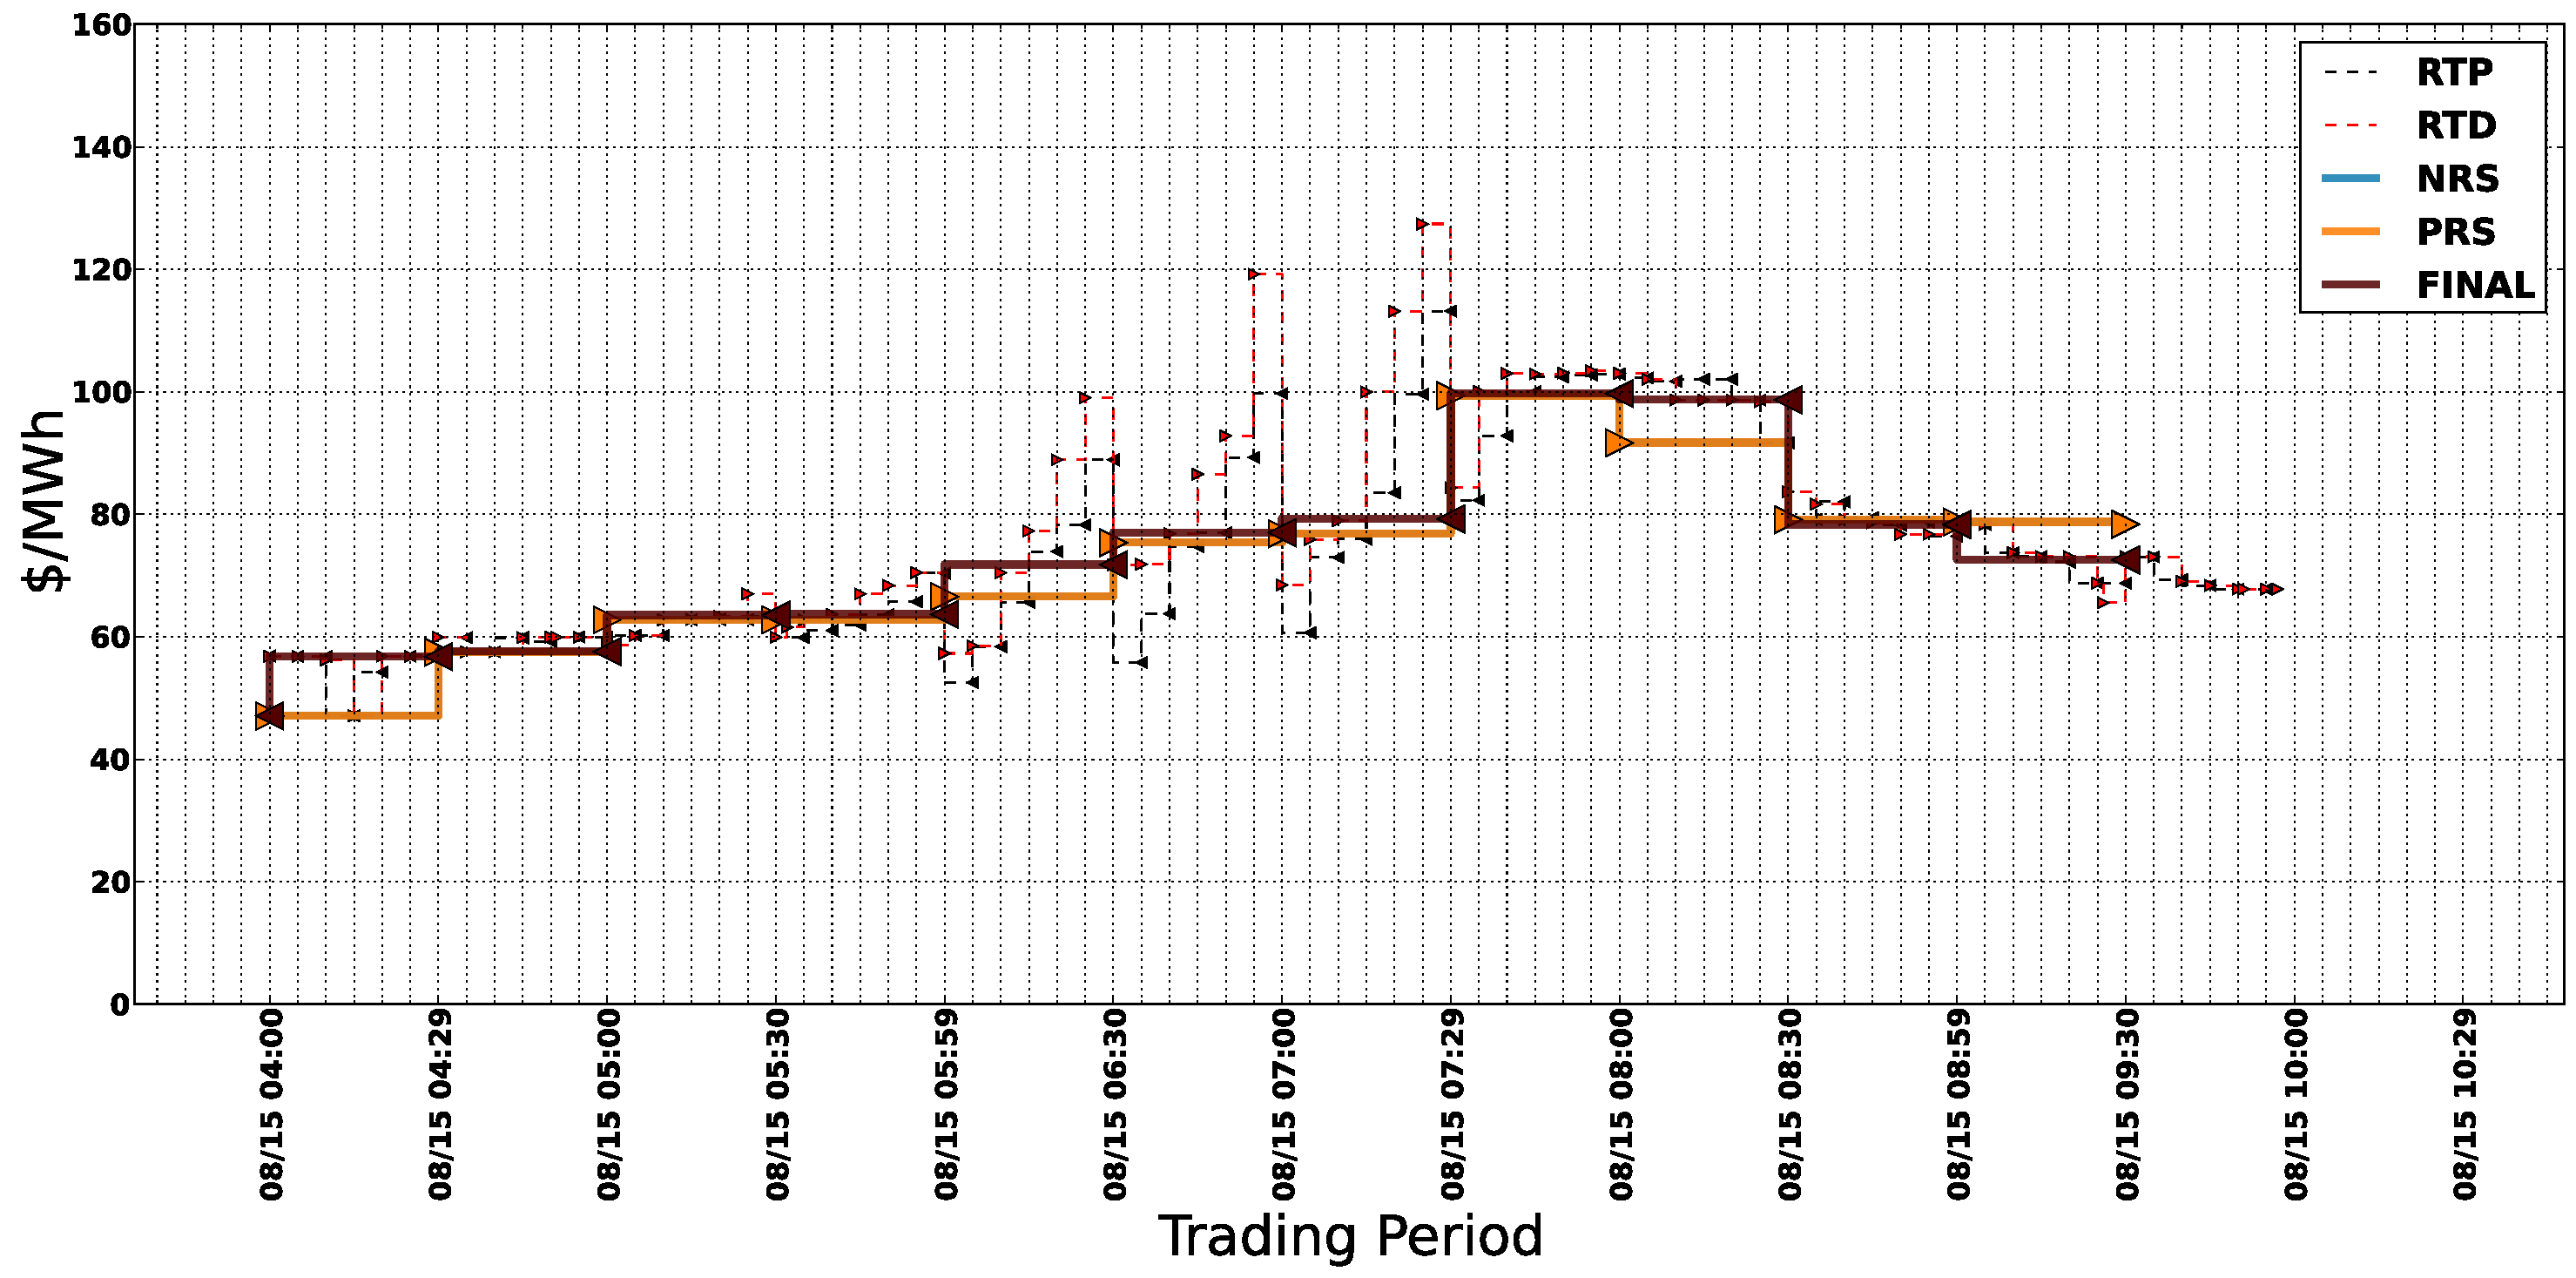
\includegraphics[width=14.5cm]{./notebooks/125_years_of_data_files/125_years_of_data_fig_06.pdf} 
\end{center}
}

\begin{frame}[fragile]
  \frametitle{POCP monitoring}

\begin{itemize}
   \item POCP $=$ Planned Outage Co-ordination Process (POCP) 
   \item database run by the System Operator
   \item a voluntary platform where participants can publish intended planned generation and transmission outages
   \item jointly developed by participants over 10 years ago  
   \item currently under review by WAG/SO 
   \item \url{http://nzeb.redspider.co.nz/} graphical interface + custom alerts etc.  
   \item great for future planning, and outage assessment
   \item not-so-great for inspecting historic outages.   
   \item a few issues with the way the current POCP database is setup\ldots 
\end{itemize}

\end{frame}


\frame
{\frametitle{POCP monitoring}
\begin{center}
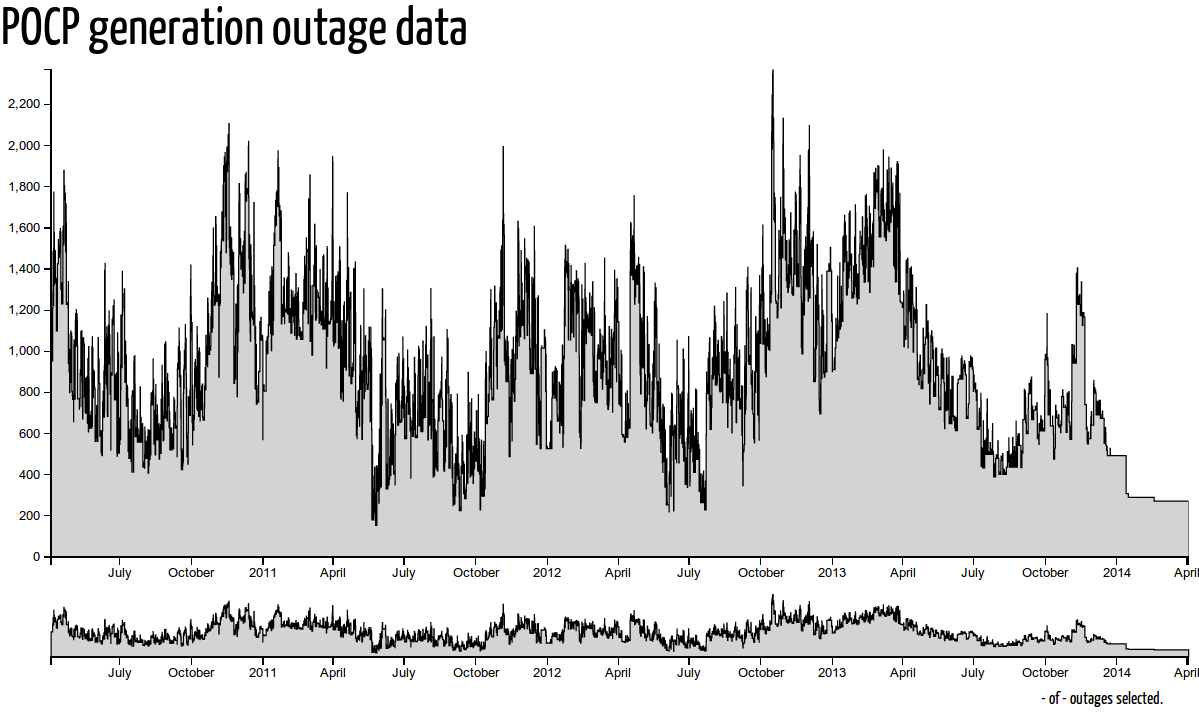
\includegraphics[height=8cm]{pocp1.png} 
\end{center}
}

\frame
{\frametitle{POCP monitoring}
\begin{center}
\includegraphics[height=8cm]{pocp_ni.png} 
\end{center}
}

\frame
{\frametitle{POCP monitoring}
\begin{center}
\includegraphics[height=8cm]{pocp_si.png} 
\end{center}
}

\frame
{\frametitle{POCP monitoring}
\begin{center}
\includegraphics[height=8cm]{pocp_now.png} 
\end{center}
}

\frame
{\frametitle{Open Source Software}

\begin{flushright}
\includegraphics[height=1cm]{IPy_header.png} 
\end{flushright}
\vspace{-5mm}
\begin{itemize}
   \item paper/presentation based entirely on open-source, freely available software
   \item iPython notebook, interactive Python development within web-browser
   \item iPython with Numpy/Pandas used daily, replaced Matlab, Excel and R.
   \item browser based interactive visulisation growing extremely quickly
   \item Javascript/d3 leading the pack.
\end{itemize}
\includegraphics[height=1cm]{download.jpg} 

}

\frame
{\frametitle{Thanks -- questions?}

\vspace{20mm}
\emph{\ldots On Wednesday the 24'th of November 1886, bright light had been brought to the bars of Dawson's, Kater's, Stevenson's and William's hotels by showman Walter Prince via underground cable through attaching a one kilowatt generator to the Oxley's brewery's steam engine. The test required regular visits of the spectators between the hotel and the brewery, and there was high demand at each point of supply. As a result, many were carrying an overload and it was not only the hotel that was lit up.\ldots''}
\begin{flushright}
\scriptsize from `Electrical development in New Zealand' \\
H.J. Beech
\end{flushright}
}

\end{document}
    
